\section{Entwurf einer Besiedlungsgeschichte des Kongobeckens}\label{sec:Zeitscheiben}	

Der aus der Zusammenschau der diskutierten regionalen Sequenzen (Kap.~\ref{sec:ICB_StilGrDatierungen}--\ref{sec:NordCongo}) entwickelte Entwurf eines Chronologieschemas für das Kongobecken (Abb.~\ref{fig:Chronologiesystem}) spiegelt eine Reihe kulturhistorischer Entwicklungen wider, die im Folgenden detailliert diskutiert werden. Die knapp 2500~Jahre umspannende keramische Entwicklungsgeschichte der Region wird dafür in drei Perioden unterteilt: eine vom Beginn der Besiedlung im 4.~Jh. v.~Chr. bis in das 6.~Jh. n.~Chr. reichende frühe Eisenzeit\footnote{Erneut folgt diese Arbeit der an anderer Stelle etablierten Systematik \parencite[74--75]{Eggert.2016d} und greift nicht auf eine zusätzliche Phase zwischen der jüngeren Steinzeit (\textit{Late Stone Age}) und der frühen Eisenzeit zurück. Siehe auch Anm.~\ref{ftn:ShumLaka} und \ref{ftn:Neolithikum}.}, eine vom 7.--11.~Jh. n.~Chr. datierende mittlere Eisenzeit und schließlich die ab dem 12.~Jh. n.~Chr. bis in die Gegenwart andauernde späte Eisenzeit.\footnote{Aus dem untersuchten keramischen Inventar des nordwestlichen Kongobeckens liegen keine dezidierten europäischen Importfunde vor; daher wird eine historische Periode, wie sie beispielsweise in Gabun beobachtet werden kann (Kap.~\ref{sec:Gabun}), nicht abgegrenzt. Sie ließe sich potenziell erst mit der Erschließung des Kongobeckens durch die europäischen Kolonialmächte in der zweiten Hälfte des 19.~Jh. n.~Chr. postulieren. Ein direkter Einfluss auf die Entwicklung der lokalen Töpfereitraditonen kann gegenwärtig nicht beobachtet werden.} Die frühe wie späte Eisenzeit kann jeweils noch in drei Stufen untergliedert werden. Dieser Entwurf einer Periodisierung ist als eine provisorische chronologische Differenzierung anzusehen und dient als Diskussionsbasis, um potenziell zeitgleiche Phänomene betrachten zu können. Aussagen im Sinne einer entwicklungsgeschichtlichen Kulturklassifikation lassen sich nicht daraus ableiten \parencite[siehe][40--43]{Eggert.2012e}.\footnote{So lässt sich die \textit{Ablösung} von flachbodiger durch rundbodige Keramik sowie das Aufkommen von Rouletteverzierung nur sehr begrenzt als entwicklungsgeschichtlicher Marker im Sinne einer Kulturklassifikation diskutieren, da es sich lediglich um diagnostische Eigenschaften der Keramik handelt.} Die folgende Diskussion des Besiedlungsgangs im Kongobecken gründet auf den Erkenntnissen aus dem von \textcite{Wotzka.1995} aufgearbeiteten Inventaren aus dem Inneren Kongobecken, ersten Ergebnissen aus dem nordöstlichen Kongobecken \parencite{LivingstoneSmith.2017} sowie den in der vorliegenden Arbeit gewonnenen Erkenntnissen zum nordwestlichen Kongobecken.\footnote{Die Kartierungen (Abb.~\ref{fig:EIA1_Karte}--\ref{fig:LIA3_Karte}) decken das Kongobecken zwischen 6$^\circ$~Nord und 2$^\circ$~Süd sowie 15$^\circ$~Ost bis 26$^\circ$~Ost an. Es wurden nur solche Fundstellen kartiert, an denen eine spezifische Stilgruppe sicher nachgewiesen wurde. Fundstellen aus dem Arbeitsgebiet, an denen eine Stilgruppe nur unter Vorbehalt nachgewiesen wurde, sind in den Verbreitungskarten in Kap.~\ref{sec:Keramiksequenz} verzeichnet.}

\paragraph{Ältere Phase der frühen Eisenzeit (4.--2.~Jh. v.~Chr.)}\hspace{-.5em}|\hspace{.5em}%
Die früheste keramische Entwicklung im Inneren Kongobecken ist durch die Imbonga-Keramik \parencite[59--68]{Wotzka.1995} repräsentiert, die in das 4.--2.~Jh. v.~Chr. datiert und an 59 Fundstellen, nahezu dem gesamten westlichen Teil des von \textcite{Wotzka.1995} untersuchten Raumes, verbreitet ist (Abb.~\ref{fig:EIA1}).\footnote{Hinweise auf Eisenmetallurgie in Kontexten der Imbonga-Gruppe ergaben sich bei Grabungen des Kölner Kongoprojektes unter Leitung von H.-P.~Wotzka in Iyonda im Jahr 2015 (mündl. Mitt. Wotzka 2016).\label{ftn:EisenIYO15/2-4}} Auch im nordöstlichen Kongobecken ist ab dem 4. Jh. v.~Chr. mit keramischen Zeugnissen zu rechnen. Die an insgesamt vier Fundstellen angetroffene Keramik der ältesten Phase weist auf Basis der vorliegenden Radiokohlenstoffdatierungen eine Laufzeit bis mindestens in das 1.~Jh. n.~Chr. auf \parencite[17 Abb.~23]{LivingstoneSmith.2017}. Zwischen den beiden Gruppen, die nur vordergründig formale Ähnlichkeiten zueinander aufweisen (siehe Kap.~\ref{sec:NordCongo}), liegen etwa 400--450\,km, der östliche Teil des von \textcite{Wotzka.1995} untersuchten Raumes, der erst deutlich später aufgesiedelt wurde (Abb.~\ref{fig:LIA1}).\footnote{Gegenwärtig liegen keine Erkenntnisse zur Besiedlung entlang des Kongo zwischen der 70\,km nördlich von Mbandaka gelegenen Mündung des Lulonga und den im nordöstlichen Kongobecken liegenden, 2010 erstmals untersuchten Flussläufen vor. Neue Feldarbeiten zur Schließung dieser Quellenlücke finden zwischen 2019--2021 unter der Leitung von H.-P.~Wotzka (Köln) im Rahmen des Projektes \enquote{Mittel- bis spätholozäne Biotopgrenzen, Siedlungslimits und Verbindungskorridore im Inneren Kongobecken: Archäologie und Paläoökologie} statt. Das Projekt ist Teil des Schwerpunktprogramms \enquote{Entangled Africa: Intra-African connections between Rainforest and Mediterranean (ca. 6000 to 500 BP)} (SPP 2143) der Deutschen Forschungsgemeinschaft.} Ein verbindendes Element zwischen diesen beiden Stilen, neben der Nutzung ähnlicher Verzierungstechniken wie die in großen Teilen Zentralafrikas verbreitete Wiegebandtechnik, bildet die Beobachtung, dass die frühe Keramik des nordöstlichen Kongobeckens in Aufbautechnik hergestellt ist \parencite[16]{LivingstoneSmith.2017}. Diese Technik lässt sich aufgrund der geringen Anzahl entsprechend untersuchter Gefäße unter Vorbehalt auch für die Keramik der Imbonga-Gruppe vermuten (Kap.~\ref{sec:Herstellung}; Abb.~\ref{MKA87-102-1_Makrospuren}--\ref{MIT87-103-1_Makrospuren}). Innerhalb der rezenten Töpfereitradition des Inneren Kongobeckens ist die Aufbautechnik das allgemein vorherrschende Herstellungsverfahren.\footnote{Siehe Anm.~\ref{ftn:EthnoToepfereiInVorb}.} 

\paragraph{Mittlere Phase der frühen Eisenzeit (2.~Jh. v.~Chr. -- 2.~Jh. n.~Chr.)}\hspace{-.5em}|\hspace{.5em}%
Der Beginn der mittleren Phase der frühen Eisenzeit um 200 v.~Chr. wird einerseits durch eine Differenzierung der keramischen Stilentwicklung im Inneren Kongobecken und dem damit verbundenen Ende der Imbonga-Keramik sowie andererseits durch den Beginn einer hinreichend belegbaren Aufsiedlung des nordwestlichen Kongobeckens durch die Pikunda-Munda-Gruppe im Süden (Kap.~\ref{sec:PKM-Gr}) und die Batalimo-Maluba-Gruppe im Norden markiert (Kap.~\ref{sec:BTM-Gr}; Abb.~\ref{fig:EIA2}). Die jüngeren Ausprägungen der Imbonga-Gruppe umfassten nach \textcite{Eggert.1983} noch Merkmale, die von \textcite{Wotzka.1995} in die Stile Bonkake, Ingende und Inganda ausdifferenziert wurden.\footnote{Siehe Anm.~\ref{ftn:AufteilungIMB}.} Eine Ausweitung des Siedlungsareals im Inneren Kongobecken lässt sich nur am unteren Tshuapa, bis in die Region um Boende sowie am unteren Luilaka beobachten. Die keramische Entwicklung in den Jahrhunderten um die Zeitenwende ist vornehmlich von Regionalisierung und Differenzierung geprägt. So ist die Stilgruppe Ingende auf den äußersten Westen des von \textsc{Wotzka} (ebd. 546f. Karte~3) untersuchten Raumes, die Region um Mbandaka, beschränkt. Auch die Bokele-Gruppe ist nur an zwei Fundorten im Westen des Inneren Kongobeckens nachgewiesen (ebd. 556\,f. Karte~8). Im südlichen Teil des einstiegen Verbreitungsgebietes der Imbonga-Keramik finden sich die Stilgruppen Bonkake (ebd. 546\,f. Karte~3), Lokondola und Monkoto (ebd. 550\,f. Karte~5) sowie Lusako (ebd. 552\,f. Karte~6). Die Yete-Gruppe hat ihren Verbreitungsschwerpunkt im Bereich des Momboyo, findet sich aber ebenfalls ausschließlich im südlichen Teil des Inneren Kongobeckens (ebd. 552\,f. Karte~6). Lediglich die Inganda-Gruppe kommt nahezu im gesamten, einstigen Verbreitungsgebiet der Imbonga-Gruppe vor (ebd.548\,f. Karte~4). Im nördlichen Teil des einstigen Verbreitungsgebietes der Imbonga-Gruppe (Abb.~\ref{fig:EIA1_Karte}), entlang des Lulonga, ist eine leichte Abnahme an Fundstellen zu beobachten. Der Beginn der genannten Stile wird von \textsc{Wotzka} (ebd. 72, 77, 84) jeweils mit jüngeren Ausprägungen der Imbonga-Keramik in Zusammenhang gebracht und kann daher frühestens in das ausgehende 3./2.~Jh. v.~Chr. datieren.

\begin{figure*}[p]
	\centering
	\begin{subfigure}[b]{\textwidth}
		\centering
		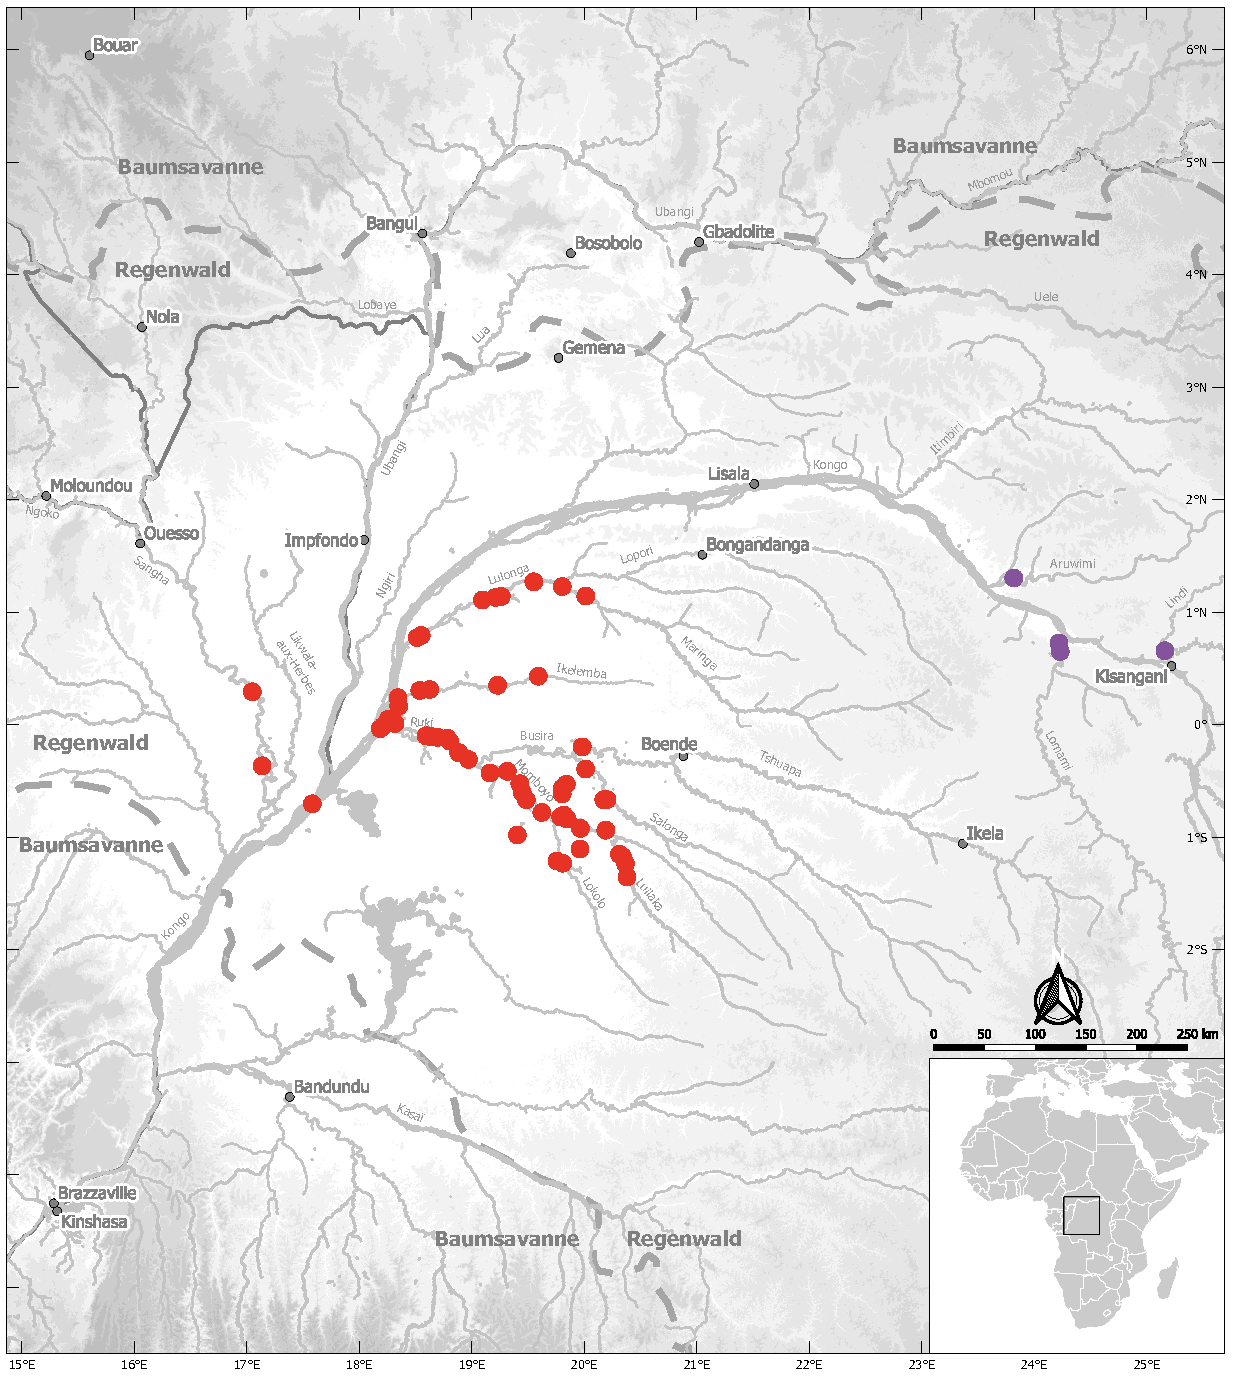
\includegraphics[width = \textwidth]{fig/5-7_Zeitscheibe_EIA1_A4print-2.pdf}
		\vspace{4cm}
		\caption{Verbreitung}
		\label{fig:EIA1_Karte}
	\end{subfigure}
	\caption{Ältere Phase der frühen Eisenzeit (4.--2.~Jh. v.~Chr.).}
	\label{}
\end{figure*}
\addtocounter{figure}{-1}
\begin{figure*}[p]
	\begin{subfigure}[b]{\textwidth}
		\setcounter{subfigure}{1}
		\centering
		\includegraphics[height = .9\textheight]{fig/Chronologiesystem_v4_Zeitscheibe_EIA1.pdf}
		\caption{Chronologie}
		\label{fig:EIA1_Chronologie}
	\end{subfigure}
	\caption{Ältere Phase der frühen Eisenzeit (4.--2.~Jh. v.~Chr.).}
	\label{fig:EIA1}
\end{figure*}

\begin{figure*}[p]
	\centering
	\begin{subfigure}[b]{\textwidth}
		\centering
		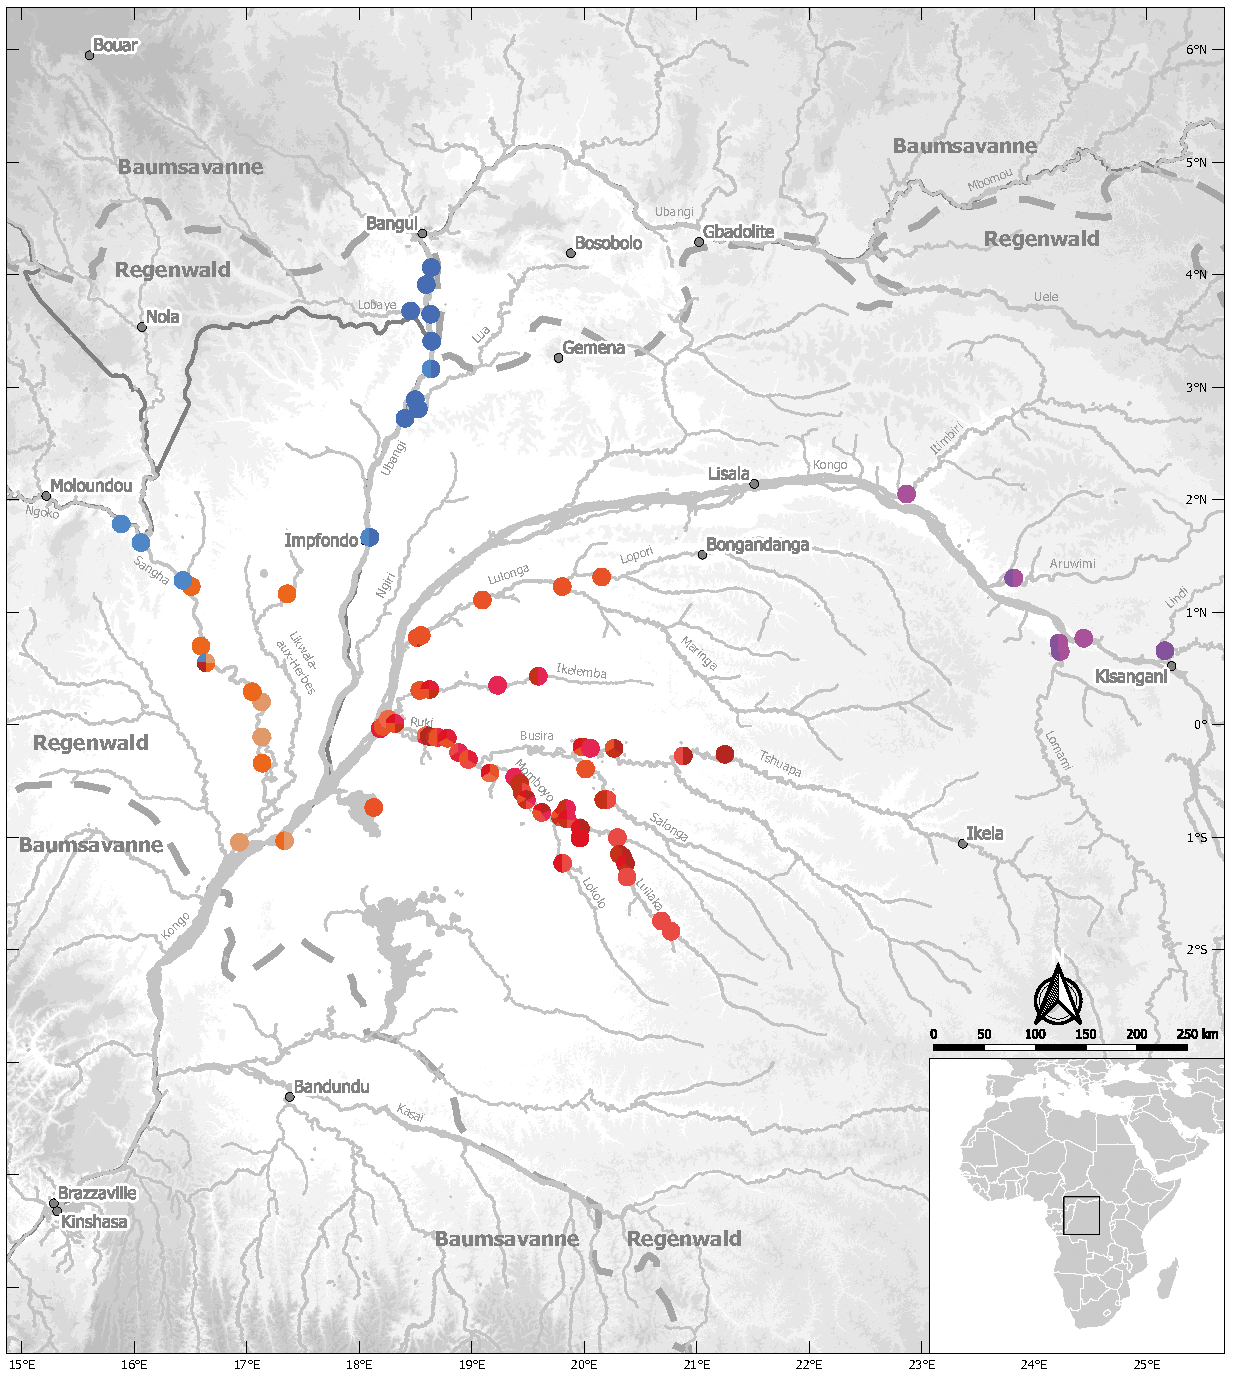
\includegraphics[width = \textwidth]{fig/5-7_Zeitscheibe_EIA2_A4print-2.pdf}
		\vspace{4cm}
		\caption{Verbreitung}
		\label{fig:EIA2_Karte}
	\end{subfigure}
	\caption{Mittlere Phase der frühen Eisenzeit (2.~Jh. v.~Chr. -- 2.~Jh. n.~Chr.).}
	\label{}
\end{figure*}
\addtocounter{figure}{-1}
\begin{figure*}[p]
	\begin{subfigure}[b]{\textwidth}
		\setcounter{subfigure}{1}
		\centering
		\includegraphics[height = .9\textheight]{fig/Chronologiesystem_v4_Zeitscheibe_EIA2.pdf}
		\caption{Chronologie}
		\label{fig:EIA2_Chronologie}
	\end{subfigure}
	\caption{Mittlere Phase der frühen Eisenzeit (2.~Jh. v.~Chr. -- 2.~Jh. n.~Chr.).}
	\label{fig:EIA2}
\end{figure*}

Im nordwestlichen Kongobecken sind frühestens ab dem 2.~Jh. v.~Chr. -- in Gestalt der Stile Batalimo-Maluba (Kap.~\ref{sec:BTM-Gr}) und Pikunda-Munda (Kap.~\ref{sec:PKM-Gr}) -- hinreichend umfassende keramische Inventare nachweisbar. Zwar liegen vom Unterlauf des \mbox{Sangha} zwei Nachweise für ältere Imbonga-Keramik vor (Abb.~\ref{fig:EIA1_Karte}), jedoch ist einerseits der Kontext dieser Funde unklar und andererseits lassen sich auch in den Surveyfunden anderer Fundstellen keine potenziell der Imbonga-Gruppe zuordenbaren Stücke identifizieren (Kap.~\ref{sec:IMB-Gr}). Die erste eindeutig fassbare Besiedlung des nordwestlichen Kongobeckens durch keramikproduzierende Gruppen erfolgte vielmehr getrennt voneinander, in zwei potenziell naturräumlich unterschiedlichen Regionen.\footnote{Acht der neun bekannten, sicher Funde der Batalimo-Maluba-Gruppe aufweisenden Fundstellen liegen außerhalb des für die Regenwaldkrise des 1.~Jt. v.~Chr. von \textcite[7 Abb.~4]{Maley.2001} postulierten Regenwaldrefugiums. Auch mit Blick auf die heutige Vegetation befinden sich die Fundstellen der Batalimo-Maluba-Gruppe am nördlichen Rand des äquatorialen Regenwaldes. Dass es sich bei den Trägern der Batalimo-Maluba-Keramik folglich nicht um Bewohner des Regenwaldes handelte, kann zwar als Hypothese angesehen werden, bedarf aber weiterer Untersuchungen. Das Verbreitungsgebiet der im südlichen Teil des nordwestlichen Kongobeckens entlang des unteren \mbox{Sangha} sowie des \mbox{Likwala}-\mbox{aux}-\mbox{Herbes} verbreiteten Pikunda-Munda-Keramik liegt heutzutage in ausgedehnten Sumpfwäldern (siehe Abb.~\ref{fig:PalaeoumweltArch_Karte}). Alle mit Pikunda-Munda-Keramik sicher zu assoziierenden Fundstellen liegen innerhalb des von \textsc{Maley} (ebd. 7 Abb.~4) postulierten Regenwaldrefugiums, das hauptsächlich das Innere Kongobecken abdeckt. Es kann davon ausgegangen werden, dass die die Pikunda-Munda-Keramik tragenden Bevölkerungen, wie auch die zeitgleichen Gruppen im benachbarten Inneren Kongobecken, im sich von der Regenwaldkrise des 1.~Jt. v.~Chr. erholenden äquatorialen Regenwald siedelten \parencite[siehe][337]{Hubau.2013}. Entlang des nordwestlichen Randes des von \textcite{Maley.2001} im Inneren Kongobecken postulierten Regenwaldrefugiums findet sich zeitgleich zu den Stilen Batalimo-Maluba und Pikunda-Munda auch Keramik der \mbox{Ngbanja}-Gruppe (Kap.~\ref{sec:NGB-Gr}). Der historische Naturraum dieser gegenwärtig nur unter Vorbehalt chronologisch ansprechbaren Stilgruppe muss jedoch offenbleiben.}

Die Stilgruppen Batalimo-Maluba und Pikunda-Munda weisen kaum formale Gemeinsamkeiten auf und auch in technischer Hinsicht unterscheiden sie sich stark. Dadurch kann gegenwärtig nur von einem getrennten Ursprung dieser beiden Stile ausgegangen werden. Beide Stile spiegeln deutlich unabhängige keramische Entwicklungen wider. Diese Hypothese lässt sich jedoch aufgrund des Mangels an entsprechenden Vergleichsfunden aus Bereichen außerhalb des Arbeitsgebietes gegenwärtig nicht belegen.

Im nordöstlichen Kongobecken liegen weiterhin Belege für die Keramik der ältesten Phase vor, die im 1.~Jh. n.~Chr. durch die formal andersartige Keramik der mittleren Phasen abgelöst wird, die ihrerseits noch bis in das frühe 5.~Jh. n.~Chr. nachgewiesen ist (Kap.~\ref{sec:NordCongo}; Abb.~\ref{fig:LivingstoneSmith2017_noCongoTrad}.4--7). Die Anwesenheit von Keramik der mittleren Phase in Moenge am unteren Itimbiri deutet eine den Kongo stromab gerichtete Ausbreitung des Siedlungsareals an, darf jedoch aufgrund der schwachen Quellenlage nicht überinterpretiert werden.

Mit der im Süden des nordwestlichen Kongobeckens verbreiteten Pikunda-Munda-Gruppe lassen sich erstmals eindeutige Belege für Eisenmetallurgie im Kongobecken beobachten. Neben Funden von Schlacken und Eisenobjekten in den ausschließlich Pikunda-Munda-Keramik aufweisenden Schichten der Grabung PIK~87/1 in Pikunda am mittleren \mbox{Sangha} (Kat.-Nr.~8), fand sich in Munda am oberen \mbox{Likwala}-\mbox{aux}-\mbox{Herbes} ein sicher in die ersten Jahrhunderte nach der Zeitwende zu datierender Befund der im Kontext pyrotechnischer Prozesse zu deuten ist (Kat.-Nr.~16). Diese Befunde sowie ein etwas jüngerer Verhüttungsbefund (Kat.-Nr.~18) sind bislang die ältesten Belege für die Produktion von Eisen im Kongobecken. Die erstmalige Aufsiedlung des Arbeitsgebietes durch keramikproduzierende Gemeinschaften sowie die im Anschluss an die Imbonga-Gruppe im Inneren Kongobecken zu beobachtende Differenzierung und Regionalisierung sind das charakterisierende Merkmal für den Beginn der mittleren Phase der frühen Eisenzeit im Kongobecken.

\paragraph{Jüngere Phase der frühen Eisenzeit (2.--6.~Jh. n.~Chr.)}\hspace{-.5em}|\hspace{.5em}%
Die jüngere Phase der frühen Eisenzeit setzt im Inneren Kongobecken im 2.~Jh. n.~Chr. ein und ist durch das Ende der durch die Imbonga-Keramik geprägten Stile Bonkake, Ingende und Inganda (Abb.~\ref{fig:Wotzka1995_TypenICB_EIA1}.5--10) sowie das Aufkommen der eng miteinander verbundenen Stile Lingonda (Abb.~\ref{fig:Wotzka1995_TypenICB_EIA1}.17--18) und Bokuma (Abb.~\ref{fig:Wotzka1995_TypenICB_EIA1}.20--21) gekennzeichnet. Weiterhin beschränkt sich der besiedelte Raum auf den westlichen Teil des Inneren Kongobeckens. Die Funde am für die Lingonda-Gruppe namensgebenden Fundplatz am mittleren Busira (Fpl.~65) belegen erstmals eine Aufsiedlung des Flussabschnitts zwischen der Einmündung des Salonga und der Mündung des Busira in den Ruki. Der Bokuma-Stil \parencite[556\,f. Karte~8]{Wotzka.1995} weist ein der älteren Monkoto-Gruppe ähnliches Verbreitungsgebiet auf (ebd. 550\,f. Karte~5), das auf den südlichen Teil des Inneren Kongobeckens beschränkt ist und vom Ruki im Westen bis zum Ende des befahrenen Abschnitts des Luilaka im Südosten reicht. Entlang des Lulonga sind erneut weniger Fundstellen als in der vorangegangen Phase zu verzeichnen (Abb.~\ref{fig:EIA3_Karte}). Die Keramik der jüngeren Phase der frühen Eisenzeit im Inneren Kongobecken ist weiterhin einem sukzessiven stilistischen Wandel unterworfen. So fällt die in der vorangegangen Phase zu beobachtende, langsame Abnahme der Wiegebandverzierung mit der Einführung von in \textit{banfwa-nfwa}-Technik erzielter Verzierung innerhalb der Lingonda-Gruppe zusammen.\footnote{Sie Anm.~\ref{ftn:banfwa-nfwa}.}

Im nordwestlichen Kongobecken haben die noch bis in das 5.--6.~Jh. n.~Chr. anzusetzenden, ältesten Stilgruppen Batalimo-Maluba (Kap.~\ref{sec:BTM-Gr}) und Pikunda-Munda (Kap.~\ref{sec:PKM-Gr}) weiterhin Bestand. Die Verbreitungsgebiete beider Gruppen spiegeln die zweigeteilte Besiedlungsgeschichte des Raumes wider: mit der in technischer Hinsicht stark an die Keramik des Inneren Kongobeckens angelehnten Pikunda-Munda-Keramik sowie der formal an die Oveng-Keramik aus Gabun erinnernden, technisch jedoch der Pikunda-Munda-Keramik und damit der Keramik aus dem Inneren Kongobecken entsprechenden Bokonongo-Gruppe (Kap.~\ref{sec:BOG-Gr}) im Süden (Abb.~\ref{fig:EIA3_Karte}). Im Norden findet sich weiterhin die Keramik der Batalimo-Maluba-Gruppe sowie jene der \mbox{Ngbanja}-Gruppe (Kap.~\ref{sec:NGB-Gr}). Das Aufkommen der Schamott-Magerung aufweisenden und formal an die Keramik von der Île des Mimosas erinnernden Bobusa-Gruppe (Kap.~\ref{sec:BBS-Gr}) kann, basierend auf dem Vergleich zu den genannten Funden aus dem Großraum Kinshasa, unter Vorbehalt in das 3./4.~Jh. n.~Chr. datiert werden. Die Keramik der Bobusa-Gruppe stellt ein von allen bekannten keramischen Phänomen des Kongobeckens unabhängiges Element der Besiedlungsgeschichte des Raumes dar. Gegenwärtig ist das formale Spektrum der Bobusa-Keramik zu schwach belegt und die generelle Verzierungsarmut der Stücke reduzieren den Korpus diagnostischer Merkmale weiter. Systematisch lässt sich lediglich die intentionelle Magerung mit zerstoßener Keramik anführen, die in keinem anderen Kontext im Kongobecken beobachtet werden kann.\footnote{Naturräumlich kann angeführt werden, dass sich die Fundstellen der Bobusa-Gruppe nur wenige Kilometer den Kongo stromauf der heutigen südlichen Grenze des Regenwaldes befinden. Inwieweit stromab Funde der Bobusa-Gruppe zu erwarten sind, und wo die südliche Grenze des sich potenziell noch von der Regenwaldkrise des 1.~Jt. v.~Chr. regenerierenden äquatorialen Regenwalds (Kap.~\ref{sec:Palaeoumwelt}) befand, kann mit den vorliegenden Quellen nicht beantwortet werden.}

Im nordöstlichen Kongobecken finden sich lediglich Vertreter der Keramik der mittleren Phase (Abb.~\ref{fig:LivingstoneSmith2017_noCongoTrad}.4--7; Kap.~\ref{sec:NordCongo}). Diese ist in einem Bereich von etwa 250\,km Länge zwischen den Mündungen der Flüsse Itimbiri und Lomami verbreitet. Sie zeigt keine formalen Ähnlichkeiten zu den zeitgleichen keramischen Stilen des Inneren sowie nordwestlichen Kongobeckens und muss gegenwärtig ebenfalls als eigenständige Entwicklung angesehen werden.


\paragraph{Mittlere Eisenzeit (7.--10.~Jh. n.~Chr.)}\hspace{-.5em}|\hspace{.5em}\label{sec:MIA}%
Für den Zeitraum zwischen dem 6./7. bis 11./12.~Jh. n.~Chr. liegen für weitere Teile des Kongobeckens nur sehr wenige Anzeichen einer Besiedlung in Form von datierten Keramikfunden vor. Die Projektion der Angaben zur Chronologie der jeweiligen Stilgruppen aus dem von \textsc{Wotzka} (1995) untersuchten Inneren Kongobecken auf eine absolute Zeitskala erbrachte eine auffällige Zweiteilung der dortigen Sequenz (Kap.~\ref{sec:ICB_StilGrDatierungen}): das Ende der Stilgruppen Bokuma und Lingonda fällt in das 5.--7.~Jh. n.~Chr. und das Aufkommen der Bondongo-Keramik kann nicht vor den Beginn des 11.~Jh. n.~Chr. datiert werden. Für die Zeit zwischen dem 7.--10.~Jh. n.~Chr. erwähnt \textsc{Wotzka} (ebd. 121--128) lediglich der Longa-Gruppe zuweisbare Funde (Abb. \ref{fig:14C_InnerCongo_Stylegroups}.1--3). Während der Longa-Stils einen stilistisch überbrückenden Charakter zwischen den älteren Stilen Bokuma und Bokele sowie dem jüngeren Bondongo-Stil und ihm nahestehenden Gruppen aufweist lieferten die drei mit Longa-Keramik assoziierten Radiokohlenstoffdatierungen \textsc{Wotzka} (ebd. 127\,f. mit Tab.~53) aufgrund ihrer massiven Streuung nur unzureichende absolute Datierungsindizien.\footnote{In einer 2015 entstandenen Zusammenstellung von Typentafeln für die Stilgruppen des Inneren Kongobeckens gibt Wotzka dem jüngsten, in das 12.--13.~Jh. n.~Chr. fallende Datum den Vorzug vor den beiden deutlich älteren. Siehe Anm.~\ref{ftn:fstafrikaWebStilGr-Tafeln}.} Eine \enquote*{Überbrückung} der im 6.--7.~Jh. n.~Chr. abbrechenden Sequenz zum jüngeren, im 11.--12. Jh. n.~Chr. einsetzenden Abschnitt durch den Longa-Stil kann im Lichte der aktuellen Quellenlage nur schwer aufrechterhalten werden (Abb.~\ref{fig:Chronologiesystem}).\footnote{Siehe Kap.~\ref{sec:ICB_StilGrDatierungen}.} 

\begin{figure*}[p]
	\centering
	\begin{subfigure}[b]{\textwidth}
		\centering
		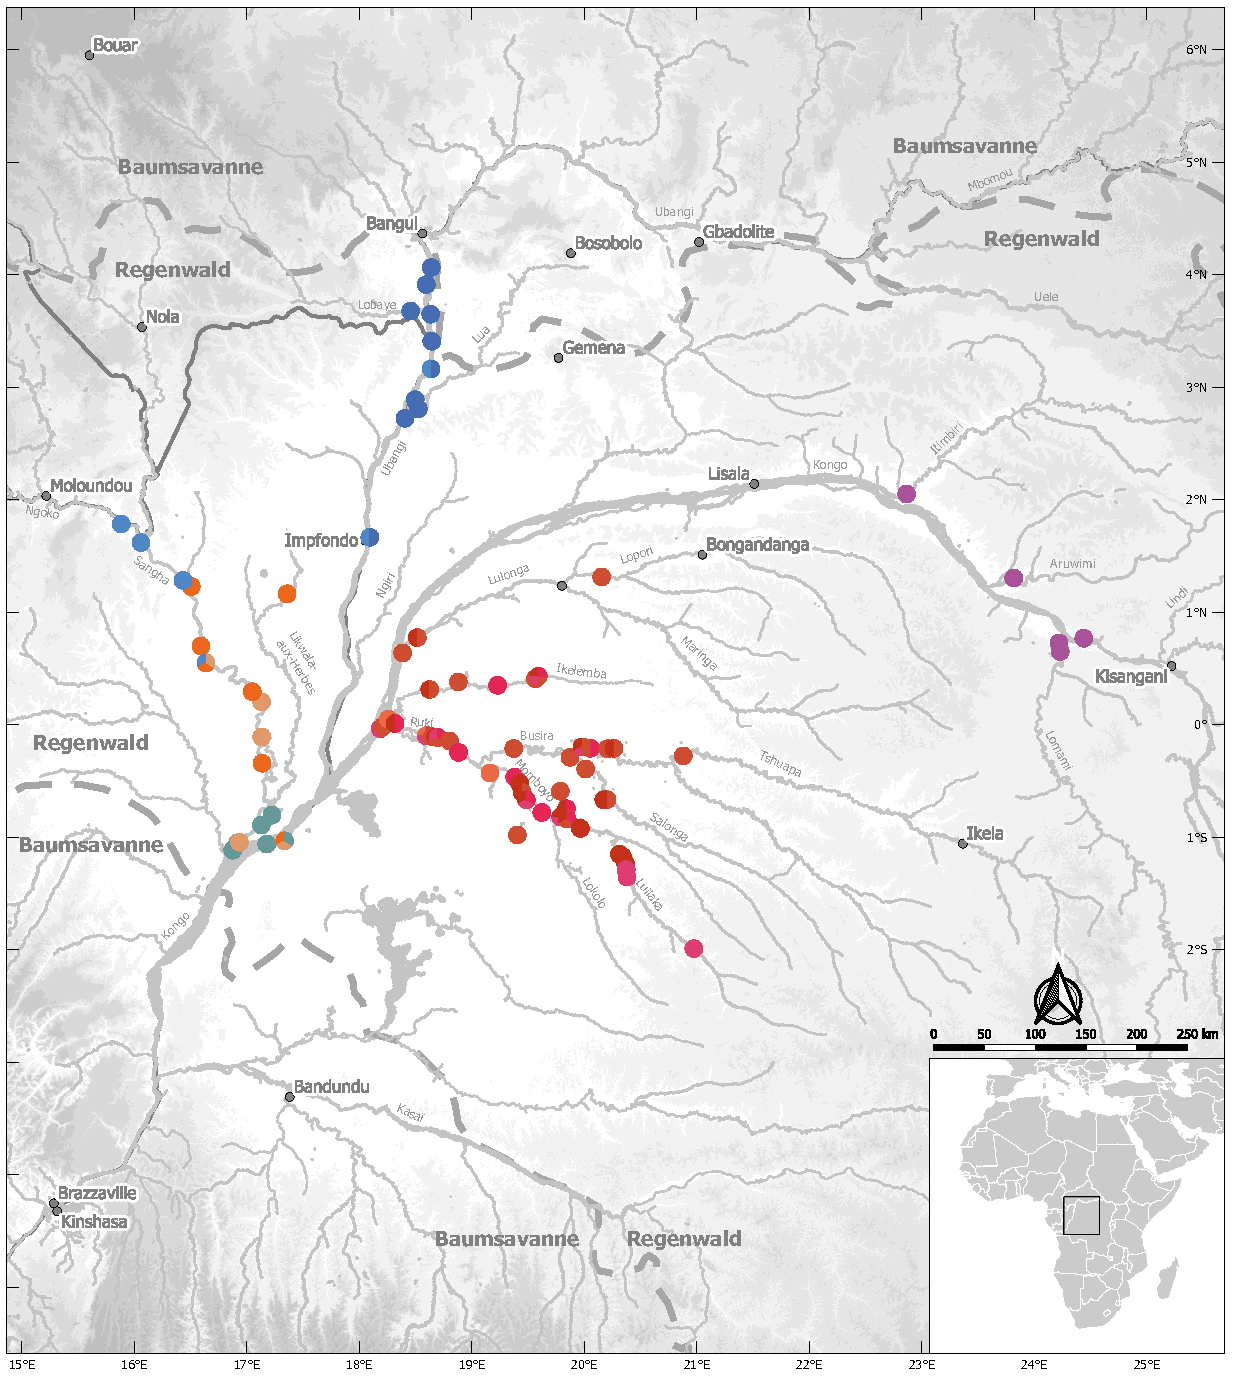
\includegraphics[width = \textwidth]{fig/5-7_Zeitscheibe_EIA3_A4print-2.pdf}
		\vspace{4cm}
		\caption{Verbreitung}
		\label{fig:EIA3_Karte}
	\end{subfigure}
	\caption{Jüngere Phase der frühen Eisenzeit (2.--6.~Jh. n.~Chr.).}
	\label{}
\end{figure*}
\addtocounter{figure}{-1}
\begin{figure*}[p]
	\begin{subfigure}[b]{\textwidth}
		\setcounter{subfigure}{1}
		\centering
		\includegraphics[height = .9\textheight]{fig/Chronologiesystem_v4_Zeitscheibe_EIA3.pdf}
		\caption{Chronologie}
		\label{fig:EIA3_Chronologie}
	\end{subfigure}
	\caption{Jüngere Phase der frühen Eisenzeit (2.--6.~Jh. n.~Chr.).}
	\label{fig:EIA3}
\end{figure*}

\begin{figure*}[p]
	\centering
	\begin{subfigure}[b]{\textwidth}
		\centering
		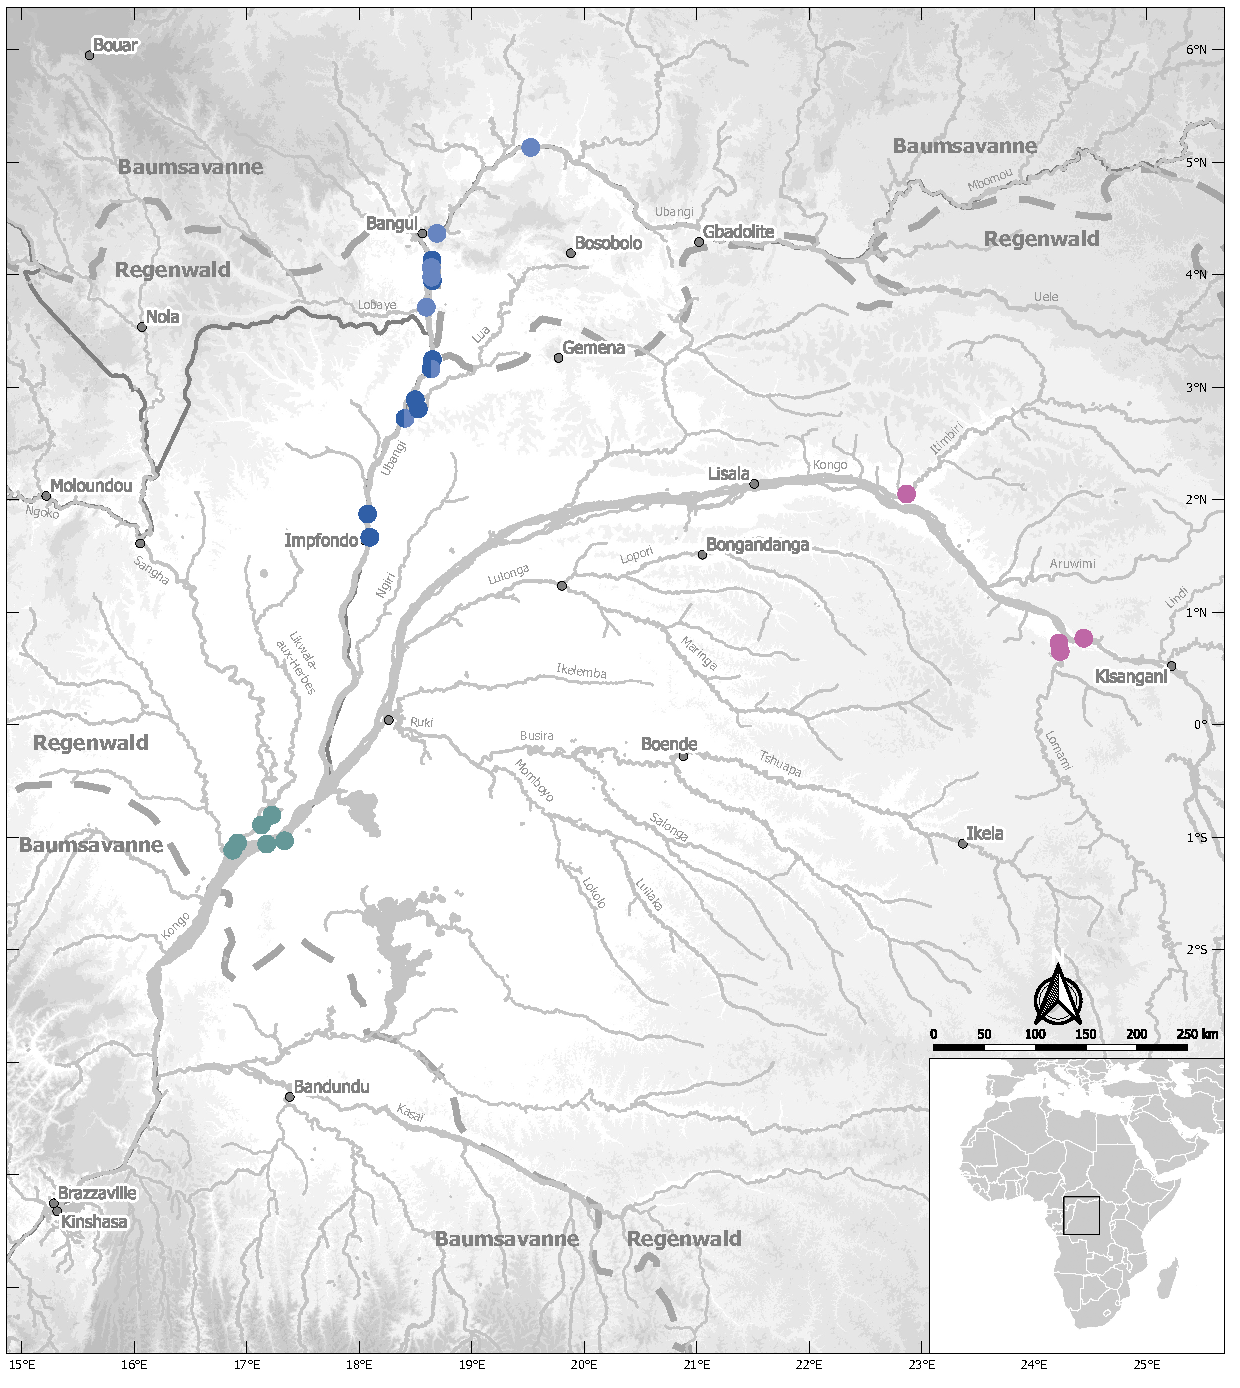
\includegraphics[width = \textwidth]{fig/5-7_Zeitscheibe_MIA_A4print-2.pdf}
		\vspace{4cm}
		\caption{Verbreitung}
		\label{fig:MIA_Karte}
	\end{subfigure}
	\caption{Mittlere Eisenzeit (7.--10.~Jh. n.~Chr.).}
	\label{}
\end{figure*}
\addtocounter{figure}{-1}
\begin{figure*}[p]
	\begin{subfigure}[b]{\textwidth}
		\setcounter{subfigure}{1}
		\centering
		\includegraphics[height = .9\textheight]{fig/Chronologiesystem_v4_Zeitscheibe_MIA.pdf}
		\caption{Chronologie}
		\label{fig:MIA_Chronologie}
	\end{subfigure}
	\caption{Mittlere Eisenzeit (7.--10.~Jh. n.~Chr.).}
	\label{fig:MIA}
\end{figure*}

Anzeiger für Aktivitäten prähistorischer Gruppen im 7.--10.~Jh. n.~Chr. sind auch im nordwestlichen Kongobecken äußerst selten. Die Nachweise für die älteren Stile Batalimo-Maluba (Kap. \ref{sec:BTM-Gr}), \mbox{Ngbanja} (Kap.~\ref{sec:NGB-Gr}), Pikunda-Munda (Kap.~\ref{sec:PKM-Gr}) und Bokonongo (Kap. \ref{sec:BOG-Gr}) brechen sämtlich im \mbox{5.--6.~Jh.} n.~Chr. ab. Am mittleren \mbox{Ubangi} können lediglich Vertreter der nicht absolut datierten Stile Dongo (Kap.~\ref{sec:DON-Gr}) und Mokelo (Kap.~\ref{sec:MKL-Gr}) provisorisch dieser Phase zugerechnet werden. Diese Ansprache gründet jedoch gänzlich in dem stilistisch überbrückenden Charakter der beiden Gruppen, die die ältere Keramik der Stile Batalimo-Maluba (Kap.~\ref{sec:BTM-Gr}) und \mbox{Ngbanja} (Kap.~\ref{sec:NGB-Gr}) mit der jüngeren Motenge-Boma-Keramik (Kap.~\ref{sec:MTB-Gr}) verbinden. Da es sich hierbei jedoch um wenige Ähnlichkeiten auf Merkmalsebene handelt, müssen diese Angaben mit höchster Vorsicht betrachtet werden und eine sichere chronologische Ansprache der beiden Stile kann nur durch zusätzliche Geländearbeit erfolgen.

Am südlichen Rand des nordwestlichen Kongobeckens, dem Mündungsbereich des \mbox{Sangha}, kann noch von einem bis in das 7.~Jh. n.~Chr. hineinreichenden Weiterbestehen der Bobusa-Keramik ausgegangen werden (Kap.~\ref{sec:BBS-Gr}). Jedoch stützt sich auch diese Ansprache lediglich auf starke technische sowie schwache formale Ähnlichkeiten zur Keramik der am Pool Malebo gelegenen Île des Mimosas (Abb.~\ref{fig:Niederkongo_Sequence}.7--9). Diese ist Teil der von \textcites{deMaret.1986}{Maret.1990} beschriebenen Gombe-Gruppe, die gegenwärtig in das 3.--7.~Jh. n.~Chr. datiert wird (Kap.~\ref{sec:Niederkongo}).

Im nordöstlichen Kongobecken enden im 4.~Jh. n.~Chr. die Belege für Keramik der mittleren Phase (Kap.~\ref{sec:NordCongo}). Jedoch lassen sich Funde der Ilambi-Gruppe mit einem in das 8.--10.~Jh. n.~Chr. datierenden Radiokohlenstoffdatum in Zusammenhang bringen \parencite[4 Tab.~1: Poz-75462]{LivingstoneSmith.2017}. Die Ilambi-Keramik zeigt ein ähnliches Verbreitungsbild wie die Keramik der ihr vorangegangen mittleren Phase. Jedoch markiert ihr Aufkommen im 8.--10.~Jh. n.~Chr. einen auffälligen Bruch in der keramischen Entwicklung der Region. Die Gefäße der älteren und mittleren Phase, die in Aufbautechnik produziert wurden und eine Verzierung aus Riefen, Rillen und Eindrücken aufweisen, werden von in Abformtechnik hergestellten und rouletteverzierten Gefäßen abgelöst (ebd.~17). Es kann beim gegenwärtigen Quellenstand nur konstatiert werden, dass der beschriebene mutmaßliche Abbruch der Siedlungsaktivität in weiten Teilen des Kongobeckens mit dem von \textcite{LivingstoneSmith.2017} beobachteten Technologiewechsel zusammenfällt.\footnote{Diachrone Betrachtungen zur Keramiktechnologie liegen lediglich für das nordöstliche Kongobecken (Kap.~\ref{sec:NordCongo}) vor, während für das nordwestliche Kongobecken lediglich ein erster, nur bedingt systematischer Einblick in die Entwicklungsgeschichte der Töpfereitechnik existiert (Kap.~\ref{sec:Herstellung}). Jedoch unterstreichen die dahingehenden Ergebnisse von \textcite{LivingstoneSmith.2017} aus dem nordöstlichen Kongobecken das Potenzial entsprechender Untersuchungen.}

Ein umfassender Rückgang oder gar Abbruch der Siedlungsaktivitäten während der mittleren Eisenzeit wurde mehrfach von \textcites[101--103~Abb.~9]{Oslisly.1998}[112\,f.~Abb.~7.9]{Oslisly.2001d}{Oslisly.2013}{Oslisly.2013b} diskutiert. Belege für in der zweiten Hälfte des 1.~Jt. n.~Chr. zu beobachtende Abbrüche lokaler oder regionaler Sequenzen sind auch aus anderen Teilen Zentralafrikas bekannt. So berichtet \textcite{Leka.2008} von einer zwischen das 1.--13.~Jh. n.~Chr. reichenden Lücke in der aus elf Radiokohlenstoffdatierungen bestehenden Sequenz für eine Reihe nördlich der kamerunischen Hauptstadt Yaoundé gelegener Fundstellen. Auch an der südöstlich von Douala, im Westen Kameruns gelegenen Fundstelle Dibamba ließen sich zwischen den im 4.~Jh. n.~Chr. endenden Befunden der frühen Eisenzeit und den ab dem 10.~Jh. n.~Chr. belegten späteisenzeitlichen Strukturen keine Befunde nachweisen \parencites{Oslisly.2008}[377--380, 379 Abb.~36.6]{GouemGouem.20102011}. Die Sequenz der vor Äquatorialguinea gelegenen kleinen Insel Corisco weist ebenfalls eine auffällige Lücke auf (Kap.~\ref{sec:Gabun}). \textcite[355\,f.]{SanchezElipe.2016} weisen explizit darauf hin, dass aus dem Zeitraum zwischen dem Ende der späten Oveng-Keramik im 8.~Jh. n.~Chr. und dem Aufkommen der Nandá-Keramik ab dem 10./11.~Jh. n.~Chr. weder Gräber noch Siedlungsbefunde bekannt sind. Sie gehen für diese drei Jahrhunderte sogar davon aus, dass die Insel unbewohnt war.\footnote{Aus dem Umfeld des Gräberfeldes von Campo in Südwestkamerun liegen Radiokohlenstoffdatierungen aus Befunden vor, die bei Prospektionen nördlich der Hauptfundstelle erschlossenen wurden. Sie fallen durchweg in das 5.--7.~Jh. n.~Chr., während die Hauptbelegungszeit des erfassten Teils des Gräberfeldes im 5.~Jh. n.~Chr. endet \parencite[62\,f. Abb.~4.1]{Seidensticker.2016}.}

Eine gänzlich andere Auffassung vertreten \textcite{Lupo.2018}. Die Autoren sehen im Korpus an verfügbaren absoluten Datierungen aus dem Südwesten der Zentralafrikanischen Republik keine hinreichend überzeugenden Anzeiger für einen weiträumigen Rückgang beziehungsweise den von \textcites[101--103~Abb.~9]{Oslisly.1998}[112\,f.~Abb.~7.9]{Oslisly.2001d}{Oslisly.2013}{Oslisly.2013b} postulierten \enquote{Hiatus}. Die von anderen Autoren gezogenen Rückschlüsse aus Ballungen verfügbarer Radiokohlenstoffdatierungen auf die Demographie prähistorischer Gemeinschaften wird von \textsc{Lupo} et al. (ebd. 13--16) strikt abgelehnt.\footnote{Indem sie die Auswirkungen der Kalibration -- genauer von Effekten aufgrund der Kalibrationskurve -- durch Kalibrierung von zufällig generierten Daten statistisch darstellen können, sind \textsc{Lupo} u.~a. (ebd. 14\,f. Abb.~5) in der Lage zu zeigen, dass Gipfel und Täler in der Wahrscheinlichkeitsverteilung zumindest teilweise auf die Kalibrationskurve zurückgehen. In der vorliegenden Arbeit wurde aus genau den von \textsc{Lupo} (ebd.~13) angeführten Gründen keine Summenkalibrierung durchgeführt. Stattdessen lag der Fokus auf der chronologischen Einordnung von keramischen Phänomenen durch relative wie absolute chronologische Indizien.} Angesichts des gegenwärtigen Quellenstandes sehen die Autoren keine Anzeichen für einen Rückgang von archäologisch fassbaren Indikatoren für prähistorische Siedlungsaktivitäten zwischen dem 1. und 2.~Jt. n.~Chr.

Gegenwärtig lässt sich nicht erklären, ob und wodurch sich der mutmaßliche Rückgang an archäologischen Zeugnissen zwischen dem 7.--10.~Jh. n.~Chr. manifestiert. Von \textcite[282]{Wotzka.2006b} wird der Rückgang an Radiokohlenstoffdatierungen aus archäologischen Kontexten mit einer massiven Erholung des Regenwaldes in Zusammenhang gebracht, während \textcite{Clist.1995} lediglich ein fehlendes Forschungsinteresse verantwortlich macht. \textcite[236\,f.]{Clist.2018a} bekräftigt seine grundsätzliche Kritik an einem Rückgang archäologischer Quellen und weist explizit auf die Lücken in der Quellenlage hin, insbesondere das Fehlen von archäologischer Forschung in vielen Regionen. Während die vorliegende, gründliche chronologische Zusammenstellung von eindeutig beschriebenen keramischen Erzeugnissen in Zentralafrika eine Lücke zwischen den Töpfereiprodukten der älteren und jenen der jüngeren Eisenzeit wahrscheinlich macht (Abb.~\ref{fig:Chronologiesystem}), können über deren Ursachen nur Spekulationen angestellt werden. Neben forschungsgeschichtlichen Faktoren könnte sich auch lediglich das Siedlungsverhalten und damit die Auffindbarkeit von Zeugnissen zeitweise geändert haben. Auch ein anderes Mobilitätsverhalten, Migration oder eine grundsätzliche Populationsabnahme könnten Ursache für den Rückgang sein.

Eine Auffälligkeit ist, das der Abfall archäologischer Zeugnisse im vorliegenden Korpus an Funden und Befunden im Kongobecken zeitlich grob mit der gegenwärtig nur bedingt nachvollzogenen \textit{Late Antique Little Ice Age} beziehungsweise dem \textit{A.D. 536}-Klimaevent zusammenfällt \parencites[siehe][]{Larsen.2008}{Buntgen.2016}. Das Ende des Rückgangs archäologischer Zeugnisse im 10./11.~Jh. n.~Chr. fällt mit der Hauptphase der \textit{Medival Climat Anomaly} zusammen \parencites{Luning.2017}{Luning.2018}. \textcite[337]{Hubau.2013} beschreiben für den Zeitraum im Anschluss an das Ende der \textit{Regenwaldkrise} des 1.~Jt. v.~Chr. (siehe Kap.~\ref{sec:Palaeoumwelt}) eine Regenerationsphase des Regenwaldes im Zuge eines zunehmend feuchteren, stabilen Klimas. Während die Wechselwirkungen zwischen Vegetation und Klima für die kurzen Zeitskalen zwischen dem 7.--10.~Jh. n.~Chr. bislang nur unzureichend untersucht sind, kann festgehalten werden, dass der äquatoriale Regenwald als Ökosystem einer sehr eigenen Dynamik folgt.

\begin{figure*}[p]
	\centering
	\begin{subfigure}[b]{\textwidth}
		\centering
		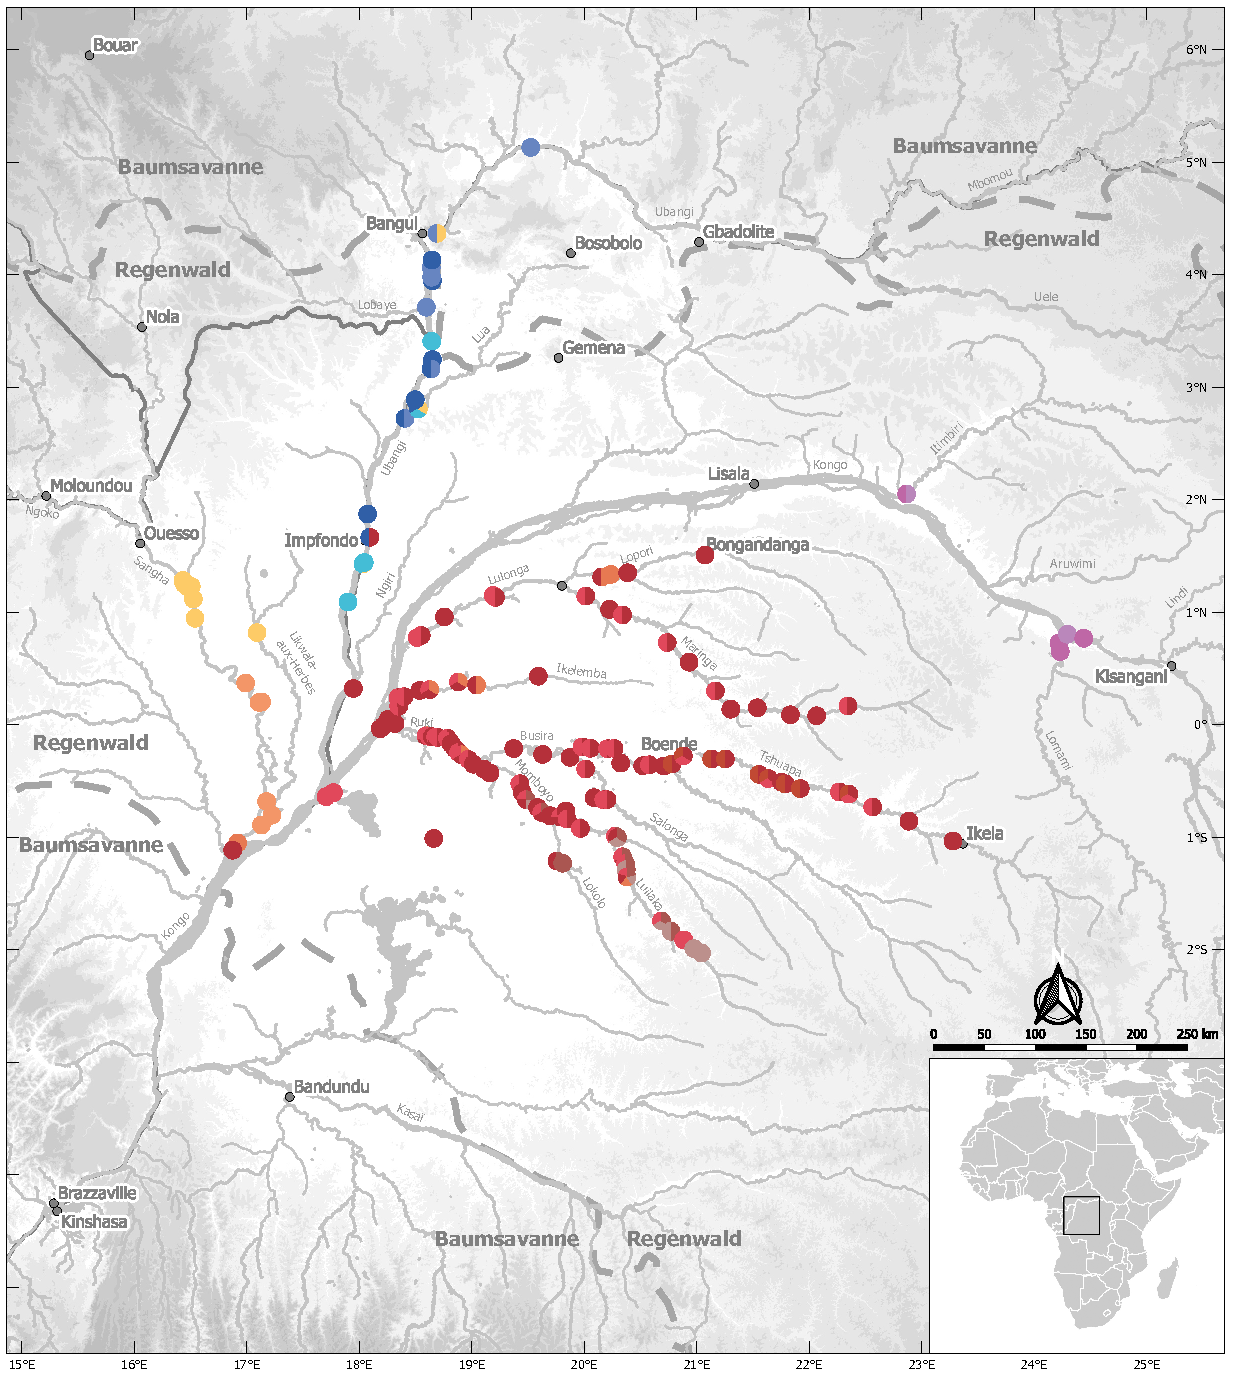
\includegraphics[width = \textwidth]{fig/5-7_Zeitscheibe_LIA1_A4print-2.pdf}
		\vspace{4cm}
		\caption{Verbreitung}
		\label{fig:LIA1_Karte}
	\end{subfigure}
	\caption{Ältere Phase der späten Eisenzeit (10.--14.~Jh. n.~Chr.).}
	\label{}
\end{figure*}
\addtocounter{figure}{-1}
\begin{figure*}[p]
	\begin{subfigure}[b]{\textwidth}
		\setcounter{subfigure}{1}
		\centering
		\includegraphics[height = .9\textheight]{fig/Chronologiesystem_v4_Zeitscheibe_LIA1.pdf}
		\caption{Chronologie}
		\label{fig:LIA1_Chronologie}
	\end{subfigure}
	\caption{Ältere Phase der späten Eisenzeit (10.--14.~Jh. n.~Chr.).}
	\label{fig:LIA1}
\end{figure*}

\begin{figure*}[p]
	\centering
	\begin{subfigure}[b]{\textwidth}
		\centering
		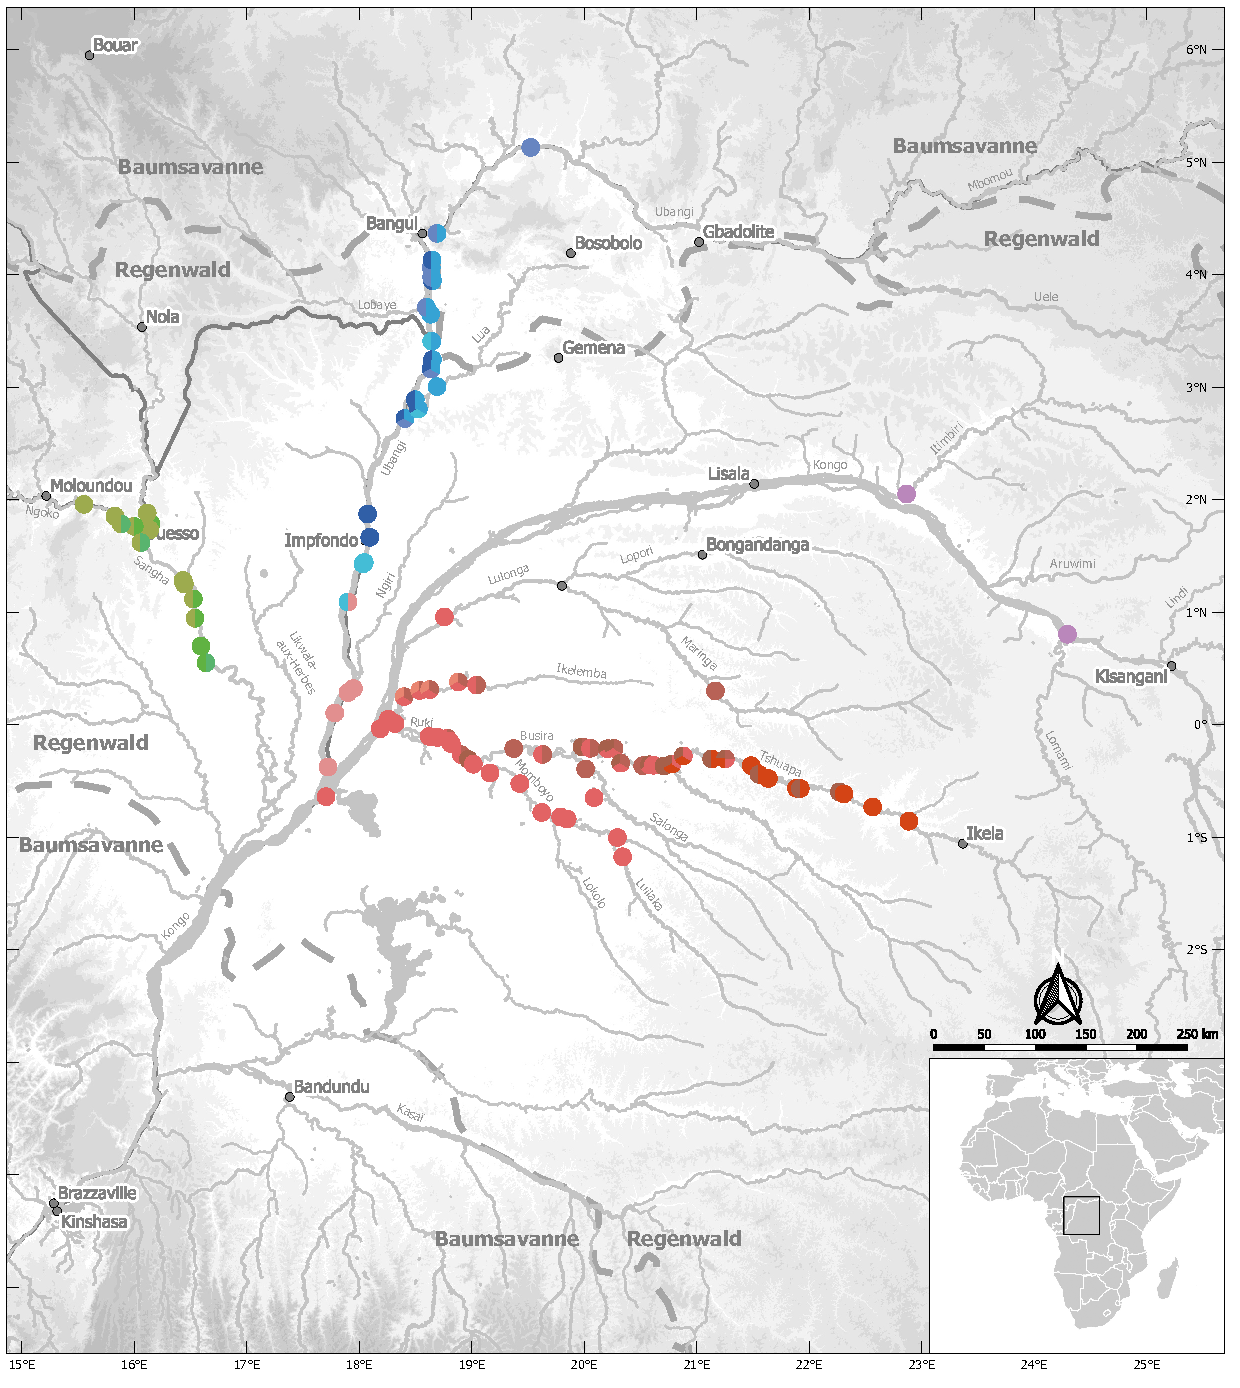
\includegraphics[width = \textwidth]{fig/5-7_Zeitscheibe_LIA2_A4print-2.pdf}
		\vspace{4cm}
		\caption{Verbreitung}
		\label{fig:LIA2_Karte}
	\end{subfigure}
	\caption{Mittlere Phase der späten Eisenzeit (14.--16.~Jh. n.~Chr.).}
	\label{fig:}
\end{figure*}
\addtocounter{figure}{-1}
\begin{figure*}[p]
	\begin{subfigure}[b]{\textwidth}
		\setcounter{subfigure}{1}
		\centering
		\includegraphics[height = .9\textheight]{fig/Chronologiesystem_v4_Zeitscheibe_LIA2.pdf}
		\caption{Chronologie}
		\label{fig:LIA2_Chronologie}
	\end{subfigure}
	\caption{Mittlere Phase der späten Eisenzeit (14.--16.~Jh. n.~Chr.).}
	\label{fig:LIA2}
\end{figure*}

\paragraph{Ältere Phase der späten Eisenzeit (11.--14.~Jh. n.~Chr.)}\hspace{-.5em}|\hspace{.5em}%
Im Anschluss an die geschilderte potenzielle Abnahme oder sogar Unterbrechung der Siedlungsaktivität während der mittleren Eisenzeit können ab dem 11.~Jh. n.~Chr. wieder eindeutige Zeugnisse einer breiten Aufsiedlung des Kongobeckens beobachtet werden. Im Inneren Kongobecken wird diese vor allem durch die nahezu im gesamten von \textcite{Wotzka.1995} bearbeiteten Raum verbreitete Stilgruppe Bondongo (ebd. 562\,f. Karte~11; Abb.~\ref{fig:Wotzka1995_TypenICB_LIA1}.4--9) getragen. Dieser Stil, zusammen mit dem potenziell zeitgleichen Longa-Stil (ebd. 558\,f. Karte~9; Abb.~\ref{fig:Wotzka1995_TypenICB_LIA1}.1--3), zeichnet sich durch eine elaborierte Verzierung aus, im Fall der Bondongo-Keramik umfasst diese eine besondere Hervorhebung der häufig plastisch ausgearbeiteten Schulterpartie der Gefäße. Die Keramik zeichnet sich -- soweit die diesbezüglich untersuchten Stichproben herangezogen werden können\footnote{Siehe Kap.~\ref{sec:Herstellung2_Fabric}.} -- vor allem durch die \textit{Fabrics} 1 und 2 aus, entspricht also ohne sichtbaren Wandel der ältereisenzeitlichen Keramik. Anstatt vor allem flacher Böden werden innerhalb der Stilgruppen der Späten Eisenzeit nun vornehmlich rundbodige Gefäße hergestellt (Tab.~\ref{fig:Wotzka1995Bodenformen}).\footnote{Während die Keramik der in die jüngere Phase der frühen Eisenzeit datierenden Stilgruppen Bokuma und Lingonda noch Anteile runder Böden von unter 8\,\% aufwiesen, liegt er innerhalb der Stilgruppen Longa und Bondongo zwischen 67--70\,\% (Tab.~\ref{fig:Wotzka1995Bodenformen}). Ein vergleichbarer Wandel von flachen zu runden Böden lässt sich im nordwestlichen Kongobecken nicht beobachten. Mit Blick auf die Besiedlungsgeschichte des Inneren Kongobeckens muss jedoch der Tatsache, dass die Stilgruppen der älteren Eisenzeit durchweg flache Boden zeigen, während sich die Stile der späteren Eisenzeit zu großen Teilen durch runde Böden auszeichnen, wie sie auch für die rezenten Töpfereibelege nachgewiesen sind \parencite{Eggert.1980c}, eine nicht zu vernachlässigende Bedeutung zugesprochen werden.} Mit der beginnenden späten Eisenzeit lässt sich zunehmend eine Verzweigung der keramischen Entwicklung der von \textcite[221--223]{Wotzka.1995} beschriebenen \textit{West-Tradition} in eigenständige, lokal geprägte Stiltraditionen am Luilaka sowie Tshuapa beobachten. Die im Süden des Inneren Kongobeckens verbreitete \textit{Luilaka-Tradition} wird aus den Stilgruppen Bekongo und Wafanya gebildet. \textcite{Wotzka.1995} attestiert ihr einen eigenständigen aber kurzlebigen Charakter. Der Bekongo-Stil spiegelt eine lokale Entwicklung der Longa-Keramik wider und weist auch deutliche Ähnlichkeiten zur Bondongo-Keramik auf. Aus ihm entwickelt sich der Wanfanya-Stil. Gegen Ende des Bondongo-Stils im 13.--15.~Jh. n.~Chr. wird von Wotzka (ebd. 222\,f.) auch im Gebiet des Tshuapa, im Osten des Inneren Kongobeckens, eine einsetzende Regionalisierung beobachtet. Diese Entwicklung setzt mit dem Wema-Stil im 13.--14.~Jh. n.~Chr. ein und lässt sich bis zur rezenten Ilemba-Bokonda-Keramik nachvollziehen (Kap.~\ref{sec:ICB_StilGrDatierungen}). Die bislang ältesten publizierten Belege für die Nutzung von Eisen im Inneren Kongobecken stammen aus mit Keramik der Bondongo-Gruppe assoziierten Fundzusammenhängen (ebd. 288).\footnote{Siehe auch Anm.~\ref{ftn:EisenIYO15/2-4}} 

Im südlichen Teil des Arbeitsgebietes findet sich die Ngombe-Gruppe, die -- trotz fehlender Radiokohlenstoffdatierungen -- aufgrund ihrer starken Ähnlichkeiten zu den aus dem Inneren Kongobecken bekannten Stilen Longa und Mbandaka provisorisch in das 12.--13.~Jh. n.~Chr. datiert werden kann (Kap.~\ref{sec:NGO-Gr}). Der Ngombe-Stil spiegelt eindeutig eine lokale Entwicklungslinie der \textit{West-Tradition} des Inneren Kongobeckens wider. Keramik der am mittleren \mbox{Ubangi} und \mbox{Sangha} sowie \mbox{Likwala}-\mbox{aux}-\mbox{Herbes} verbreiteten Matoto-Gruppe fand sich lediglich in einem datierten Befund; im Zusammenhang mit der Sekundärbestattung MLB~85/1-4-3 (Kat.-Nr.~3). Dieser Befund kann auf Basis von zwei Radiokohlenstoffdatierungen in das 11.--15.~Jh. n.~Chr. datiert werden. Die Scherben des Matoto-Stils stehen mit der Verfüllung der Eingrabung in Zusammenhang und müssten folglich mindestens zeitgleich oder älter als der Befund sein. Weiter nördlich, den \mbox{Ubangi} stromauf, finden sich weiterhin die potenziell bereits seit der mittleren Eisenzeit bekannten Stile Dongo (Kap.~\ref{sec:DON-Gr}) und Mokelo (Kap.~\ref{sec:MKL-Gr}), zu denen ab der älteren Phase der späten Eisenzeit noch die Stilgruppe Bobulu (Kap.~\ref{sec:BBL-Gr}) hinzugerechnet werden kann.

Im nordöstlichen Kongobecken lässt sich mit der älteren Phase der späten Eisenzeit die sukzessive Einführung von \mbox{Roulette} beobachten (Kap.~\ref{sec:NordCongo}). Innerhalb der auf Basis zweier Radiokohlenstoffdatierungen zwischen das 8.--10.~Jh. n.~Chr. sowie 15.--17. Jh. n.~Chr. datierenden Ilambi-Keramik zeigen sich erste Hinweise auf potenzielle Rouletteverzierung. \textsc{\mbox{Livingstone} \mbox{Smith}} u.a. (2017: 17, 19 Abb.~26) sind sich jedoch unsicher, ob es sich bei den entsprechenden Verzierungselementen um ein aus mehreren hölzernen Kernen bestehendes mit Schnur umwickeltes \mbox{Roulette} oder Mattenabdruck handelt. Die potenziell jüngere Yaekela-Keramik zeichnet sich durch eine vornehmlich aus Schnitzroulette bestehende Verzierung aus. Die Gefäße der Ilambi-Gruppe wie jene der Yaekela-Gruppe zeigen, neben dem Wechsel der Verzierungspraxis, auch einen Wandel in der Herstellungstechnik an: eine Ablösung der in Aufbautechnik hergestellten Keramik der älteren Eisenzeit durch in Abformtechnik getöpferte Gefäße. Mit Blick auf den aktuellen Stand der Auswertung muss jedoch offenbleiben, ob im nordöstlichen Kongobecken der beobachtete Wandel der Herstellungstechnik auch sicher mit der Einführung von Rouletteverzierung zusammenfällt oder ob zwischen Ilambi- und Yaekela-Keramik eher eine sukzessive Übernahme stattfand.

\paragraph{Mittlere Phase der späten Eisenzeit (14.--16.~Jh. n.~Chr.)}\hspace{-.5em}|\hspace{.5em}%
Ab dem 14.~Jh. n.~Chr. lässt sich eine zusätzliche Ausdifferenzierung in den keramischen Inventaren beobachten. Von der Bondongo-Gruppe abgeleitete Stile werden von solchen abgelöst, die auf die Nkile-Gruppe zurückgehen (Kap.~\ref{sec:ICB_StilGrDatierungen}).\footnote{Die Stilgruppen Bondongo, Bekongo, Wafanya, Besongo und Wema lassen sich aufgrund jeweils charakteristischer Gefäßformen mit ausgeprägten Schulterpartien sowie Fisch- beziehungsweise Kauri-Motiven und Girlandenzier einem \textit{Bondongoid-Horizont} zuweisen. Dieser überschneidet sich zeitlich mit einem etwas jüngeren, sich durch charakteristische Kugeltopfformen auszeichnenden Stilen Nkile, Malelembe, Bosanga und Bolondo sowie Mpokioko gebildeten \textit{Nkiloid-Hoizont} \parencites[287\,f.]{Eggert.1983}[224\,f.; Kap.~\ref{sec:Horizonte}]{Wotzka.1995}.} Mit Blick auf die Verbreitungsgebiete der dem \textit{Nkiloid-Horizont} zugewiesenen Stile fällt das fast vollständige Fehlen von Fundstellen entlang des Lulonga, Lopori und Maringa auf (Abb.~\ref{fig:LIA2_Karte}). Für die vorangegangene Phase sind entlang dieser Flussläufe noch eine Vielzahl von Fundstellen belegt (Abb.~\ref{fig:LIA1_Karte}). \textsc{Wotzka} (ebd. 235 Tab.~121--122) kann für die Flussläufe lediglich übergreifende Stilzuweiseungen angeben. Daraus ergibt sich entweder eine leicht eigenständige keramische Entwicklung, in der Merkmale verschmolzen sind oder ein potenziell dynamischer Besiedlungsgang mit Auflassungsphasen an einzelnen Flussabschnitten. Im Osten des Inneren Kongobeckens, entlang des Tshuapa, hat die gleichnamige Stiltradtion weiterhin bestand, während die nur kurzlebige \textit{Luilaka-Tradition} bereits nicht mehr beobachtet werden kann.

Entlang des unteren \mbox{Ubangi} findet sich in Form der Bokwango-Keramik eine individuelle keramische Ausprägung der \textit{Äquator-Co-Tradition}, die starke formale Ähnlichkeiten zur Keramik der Stilgruppen Mbandaka und Nkile aufweist (Kap.~\ref{sec:BKW-Gr}). Weiter stromauf, am mittleren \mbox{Ubangi}, markiert das Aufkommen der Motenge-Boma-Keramik den Beginn der mittleren Phase der späten Eisenzeit. Der Stil weist ein auffällig abgegrenztes Verbreitungsgebiet zwischen der Lua-Mündung und dem \mbox{Ubangi}-Bogen auf (Kap.~\ref{sec:MTB-Gr}). Nach den vereinzelten Hinweisen auf die Nutzung von Rouletteverzierung innerhalb der Stile Dongo und Mokelo wird diese mit der Motenge-Boma-Keramik zur bestimmenden Verzierungstechnik der Keramik am mittleren und oberen \mbox{Ubangi}.\footnote{Die frühesten Nachweise für die Roulettetechnik stammen aus Westafrika und datieren in das 2.~Jt. v.~Chr. \parencite[189]{LivingstoneSmith.2007}. Im Laufe der folgenden Jahrhunderte ist eine Ausbreitung von Rouletteverzierungen über den gesamten nördlichen Sahel, vom Senegal im Westen bis in die Region der großen Seen in Ostafrika, zu beobachten (ebd. 203 Abb.~9). Frühere Studien haben in der Ausbreitung der Rouletteverzierung tiefgreifende Veränderungen für die jeweiligen Regionen gesehen und diese häufig mit der Verbreitung bestimmter linguistischer Gruppen in Zusammenhang gebracht. So wurde zum Beispiel die Ausbreitung von Schnitzroulette als materieller \textit{Marker} der Adamawa-\mbox{Ubangi}-Sprachen gewertet \parencite{David.1977}. In ihrer Analyse von linguistischen Veränderungen, genauer jener der Bezeichnungen für Gegenstände, die bei der Keramikherstellung genutzt werden, sowie archäologischen Belegen von Rouletteverzierung in der Uele-Region der Demokratischen Republik Kongo und der Karanga-Region Tansanias, spricht sich Mary \textcite{McMaster.2005} gegen die Möglichkeit aus, dass Diffusion der treibende Faktor der Ausbreitung der Rouletteverzierung gewesen sei. Bei Betrachtung der gegenwärtigen Chronologie der Einführung von Rou\-lette\-ver\-zier\-ung in der Region der großen Seen scheint aber auch eine simple Verbreitung durch Migration wenig wahrscheinlich (ebd. 63). Ungeachtet dessen sieht \textcite{McMaster.2005} in der Einführung der Rouletteverzierung einen Wendepunkt in der regionalen Besiedlungsgeschichte. Zu anderen Schlüssen kommt Ceri \textcite{Ashley.2010}, die eine keramische Übergangsphase zwischen der Urewe-Keramik, der ältesten keramischen Stilgruppe des Gebiets zwischen den großen Seen, und der jüngeren mit vegetabilischem \mbox{Roulette} verzierten Ware aufzeigen kann. Der Übergang, wie er von \textcite{Ashley.2010} beschrieben wird, vollzieht sich im 10.~Jh. n.~Chr., als weniger aufwendige, jedoch deutliche Ähnlichkeiten zur älteren Urewe-Keramik aufweisende Formen, durch nicht mit \mbox{Roulette} verzierte Formen abgelöst werden \parencite[890\,f.]{Reid.2013}. Diese werden in der ersten Hälfte des 2.~Jt. n.~Chr. durch die Entebbe-Gruppe abgelöst, die ähnliche Grundformen zeigt, aber Verzierungen mittels \textit{twisted string}-Roulette in Kombination mit breiten Rillen aufweist. Die Entebbe-Keramik leitet in der Folge zu den typischen, rouletteverzierten Formen der Region über. Für \textcite{Ashley.2010} ergibt sich durch die Einführung der Rouletteverzierung kein Bruch in der Sequenz. Im nordwestlichen Kongobecken bildet Rouletteverzierung ebenfalls ein leicht ansprechbares Charakteristikum, das jedoch kaum als Anzeiger für einen tiefgreifenden Wandel interpretiert werden kann.}

Im westlichen Teil des Arbeitsgebietes, entlang des oberen \mbox{Sangha} und \mbox{Ngoko}, schlägt sich ab dem 13./14.~Jh. n.~Chr. erstmals eine deutliche Siedlungsaktivität in den Inventaren nieder, die als \textit{\mbox{Ngoko}-Tradition} systematisiert ist (Kap.~\ref{sec:NgokoTradition}). Die älteste und einzige direkt datierte Ausprägung dieser Stiltradition stellt die Mandombe-Keramik dar, deren Fokus auf stark bauchige Gefäße mit kurzen Zylinderhälsen und auf Kammstrich und Appliqué-Mustern basierender Ornamentik keine Vorläufer im keramischen Fundgut der Region hat. Aus dieser sowie der mutmaßlich zeitgleichen bis leicht jüngeren Keramik der Konda-Gruppe sind erste Belege für die Nutzung von Rouletteverzierung bekannt (Kap.~\ref{sec:MDB-Gr}--\ref{sec:KON-Gr}). Innerhalb der mittleren Phase der späten Eisenzeit lässt sich auch am \mbox{Sangha} und \mbox{Ngoko} eine gelegentliche und nicht das Verzierungsspektrum der entsprechenden Stile bestimmende Nutzung von Rouletteverzierung beobachten. Entlang des \mbox{Ubangi} ist diese bereits mit den potenziell in die ältere Phase der späten Eisenzeit zu datierenden Stilen zu beobachten. \mbox{Roulette} wird in beiden Regionen erst in der jeweils folgenden Phase die bestimmende Verzierungstechnik: entlang des mittleren \mbox{Ubangi} innerhalb der Stilgruppe Motenge-Boma (Kap.~\ref{sec:MTB-Gr}) und am oberen \mbox{Sangha} und \mbox{Ngoko} innerhalb der in die jüngere Phase der späten Eisenzeit datierende Pandama-Gruppe (Kap.~\ref{sec:PDM-Gr}).

\begin{figure*}[p]
	\centering
	\begin{subfigure}[b]{\textwidth}
		\centering
		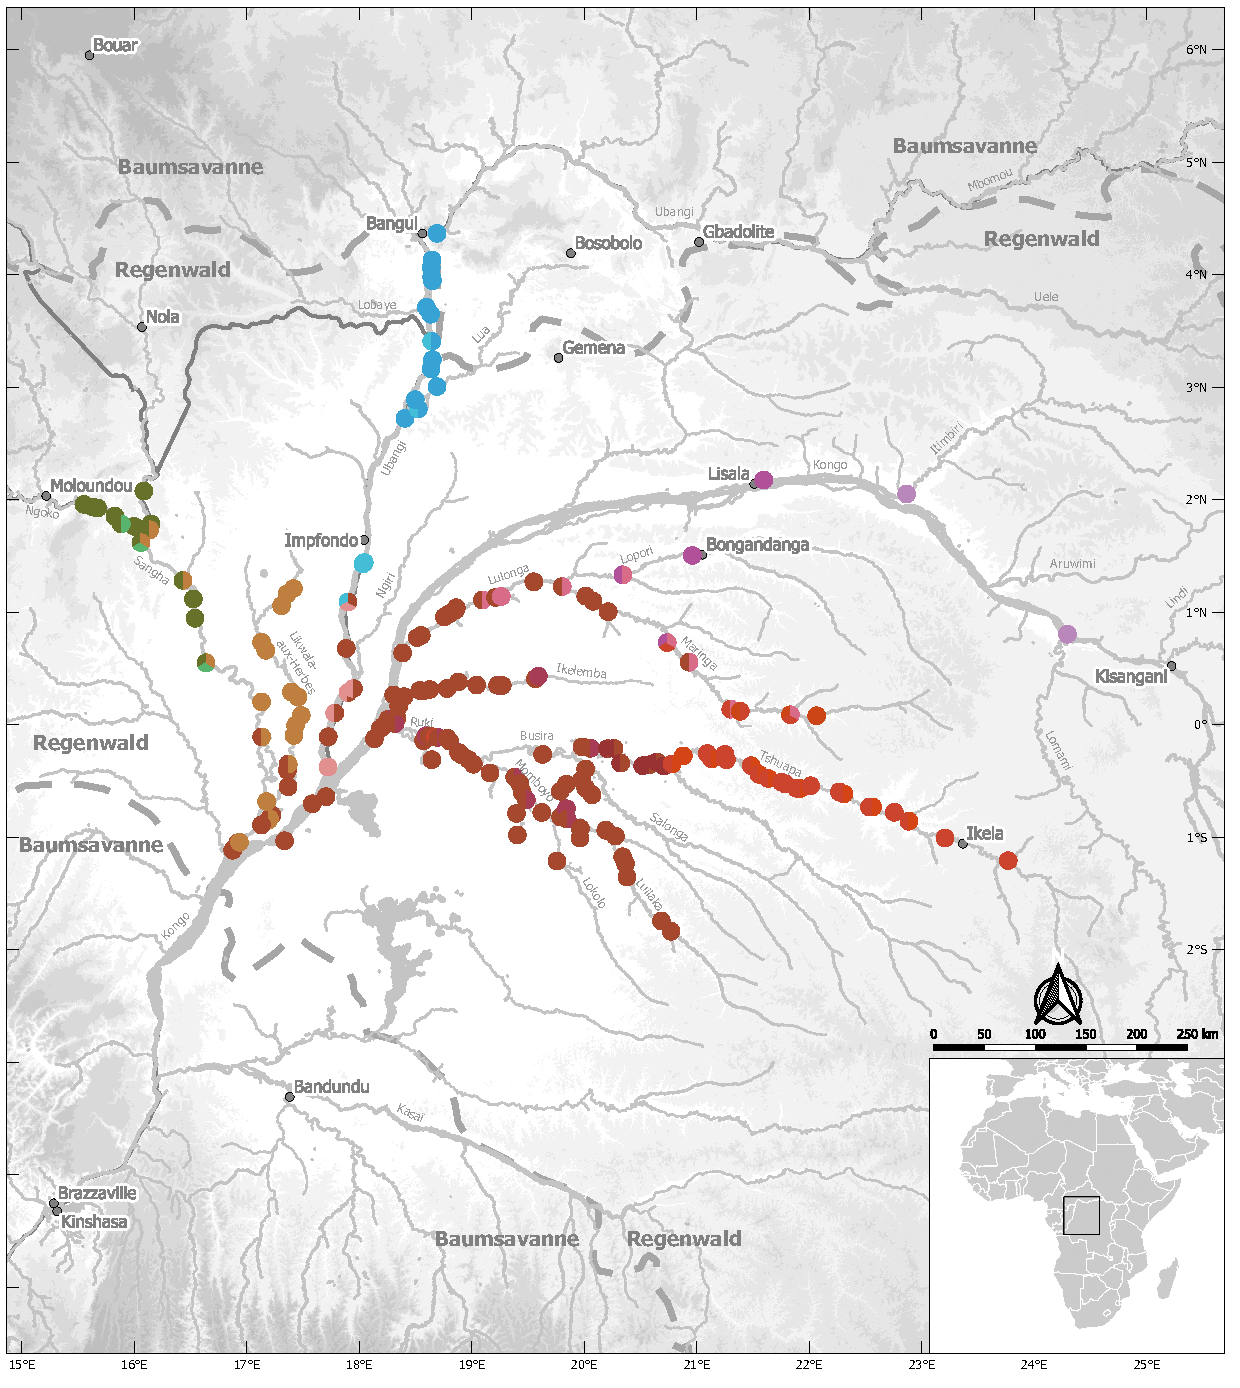
\includegraphics[width = \textwidth]{fig/5-7_Zeitscheibe_LIA3_A4print-2.pdf}
		\vspace{4cm}
		\caption{Verbreitung}
		\label{fig:LIA3_Karte}
	\end{subfigure}
	\caption{Jüngere Phase der späten Eisenzeit (17.--19.~Jh. n.~Chr.).}
\end{figure*}
\addtocounter{figure}{-1}
\begin{figure*}[p]
	\begin{subfigure}[b]{\textwidth}
		\setcounter{subfigure}{1}
		\centering
		\includegraphics[height = .9\textheight]{fig/Chronologiesystem_v4_Zeitscheibe_LIA3.pdf}
		\caption{Chronologie}
		\label{fig:LIA3_Chronologie}
	\end{subfigure}
	\caption{Jüngere Phase der späten Eisenzeit (17.--19.~Jh. n.~Chr.).}
	\label{fig:LIA3}
\end{figure*}

\begin{figure*}[p]
	\centering
	\begin{subfigure}[b]{\textwidth}
		\centering
		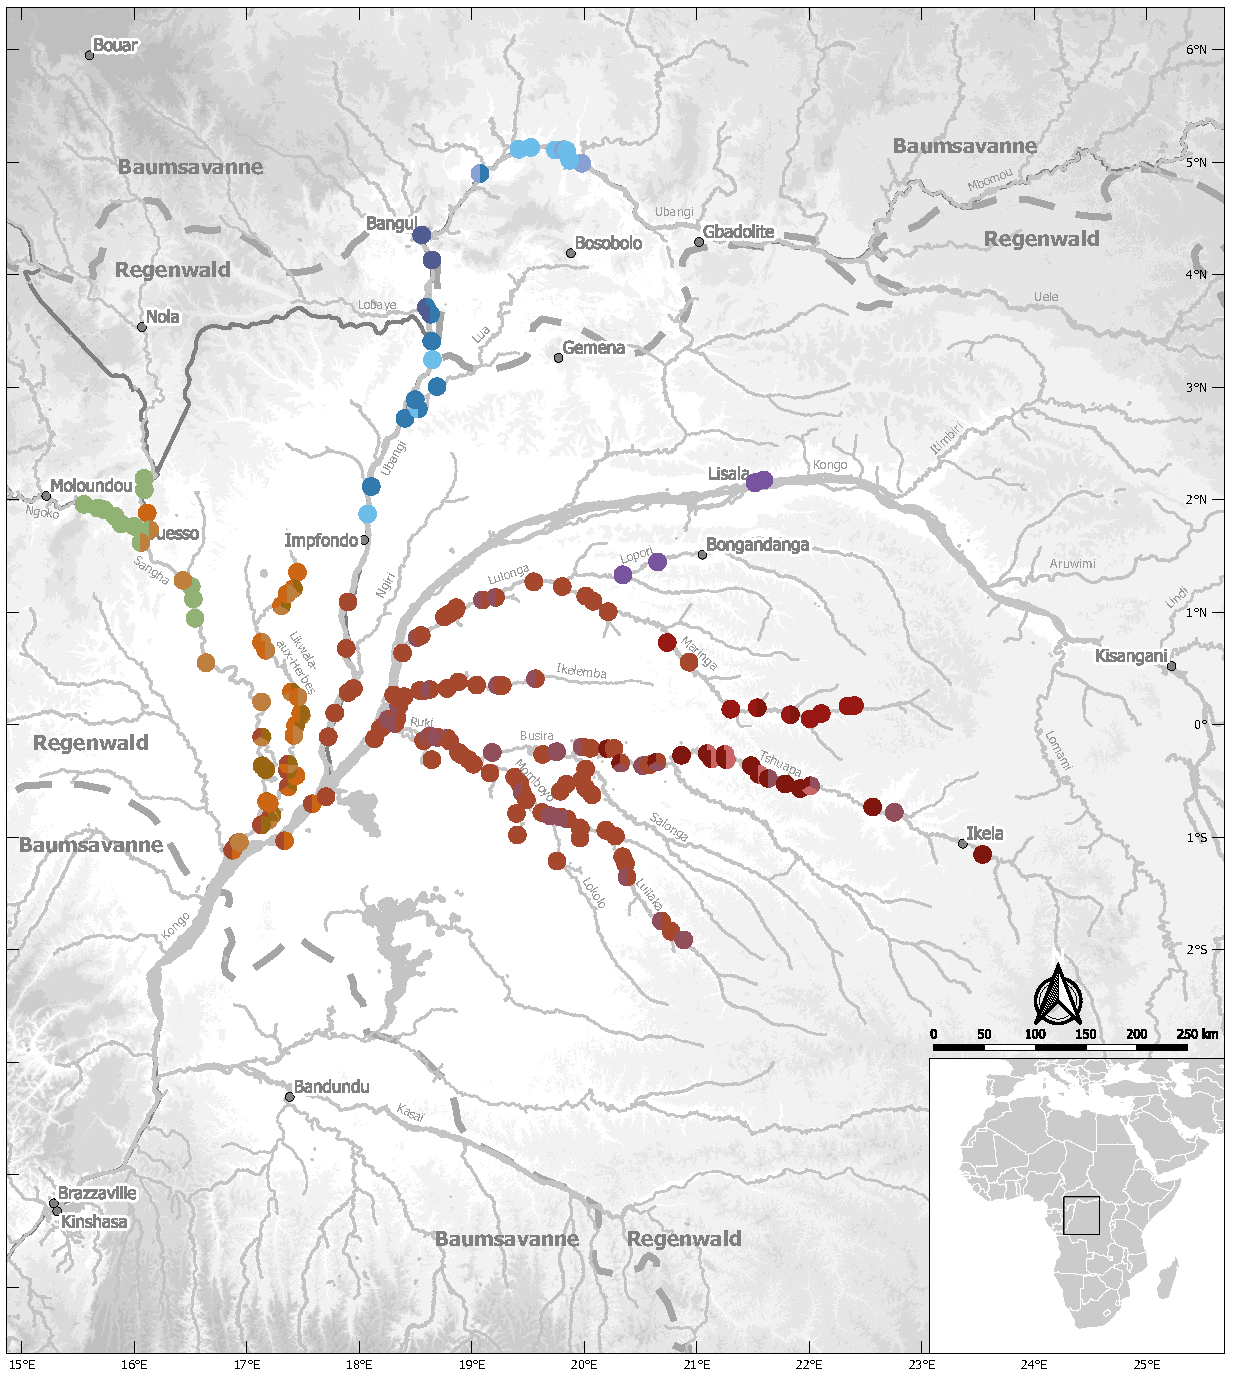
\includegraphics[width = \textwidth]{fig/5-7_Zeitscheibe_HistZeit_A4print-2.pdf}
		\vspace{4cm}
		\caption{Verbreitung}
		\label{fig:HistZeit_Karte}
	\end{subfigure}
	\caption{Historische Zeit (19.--20.~Jh. n.~Chr.).}
\end{figure*}
\addtocounter{figure}{-1}
\begin{figure*}[p]
	\begin{subfigure}[b]{\textwidth}
		\setcounter{subfigure}{1}
		\centering
		\includegraphics[height = .9\textheight]{fig/Chronologiesystem_v4_Zeitscheibe_HistZeit.pdf}
		\caption{Chronologie}
		\label{fig:HistZeit_Chronologie}
	\end{subfigure}
	\caption{Historische Zeit (19.--20.~Jh. n.~Chr.).}
	\label{fig:HistZeit}
\end{figure*}

Nachvollziehbar wird der Prozess, der mit der Einführung der Roulettekeramik in das nordwestliche Kongobecken einhergeht, unter anderem anhand des Grabungsbefundes PIK~87/1 in Pikunda am \mbox{Sangha} (Kat.-Nr. 8). Die jüngere Grube A, die bis etwa 1\,m unter die Oberfläche reicht, enthielt vornehmlich Keramik der Mandombe-Gruppe (Kap.~\ref{sec:MDB-Gr}). Diese steht formal in einem starken Kontrast zu der in der zweiten, älteren im Schnitt PIK~87/1 nachgewiesenen Grube, die fast ausschließlich Pikunda-Munda-Keramik enthielt (Kap.~\ref{sec:PKM-Gr}). Beide Gruben sind mit jeweils einer Radiokohlenstoffprobe datiert und während die Pikunda-Munda-Keramik in das 4.~Jh. v.~Chr.--3./4.~Jh. n.~Chr. datiert, stammt die Mandombe-Keramik aus dem 12.--14.~Jh. n.~Chr. Während sich die Mandombe-Keramik mit Blick auf Formen, Verzierungen und \textit{Fabrics} von der vor ihr in Pikunda nachgewiesenen Keramik der Pikunda-Munda-Gruppe unterscheidet, zeigt sie große Ähnlichkeiten zu den Stilgruppen Konda (Kap.~\ref{sec:KON-Gr}) und Pandama (Kap.~\ref{sec:PDM-Gr}). Die Ähnlichkeiten im Bezug auf die formalen Charakteristika, wie die stark bauchigen Gefäße mit kurzem Hals, und Hinweise auf eine ähnliche Technologie (Kap.~\ref{sec:Herstellung}) schließt jedoch nicht die Verzierungspraxis mit ein. Die Mandombe-Keramik zeigt vor allem diagonalen Kammstrich sowie Kammeindrücke und plastische Elemente auf den Gefäßoberteilen und häufig ein schlickergerautes Gefäßunterteil. Die Konda-Keramik hingegen weist keine plastischen Elemente oder Schlickerrauung auf. Ihre Verzierungen bestehen fast ausschließlich aus Rillen. Markant sind vor allem die innen wie außen gerillten Ränder. Sechs der Konda-Gruppe zurechenbare Stücke zeigen jedoch überdies und neben den charakteristischen Rillen auch Rouletteverzierung. Die potenziell jüngere Pandama-Keramik zeichnet sich nun regelhaft durch eine Kombination von flächigem \textit{knotted strip}-Roulette aus, welche von überkreuzten Rillen überlagert wird. Für die beiden letztgenannten Gruppen liegen keine absoluten Datierungen vor, doch weisen sie stilistisch den Weg von der Mandombe-Keramik des 12.--14.~Jh. n.~Chr. zur rezenten Mbenja-Keramik (Kap.~\ref{sec:MBJ-Gr}) und werden daher provisorisch als chronologisch zwischen diesen beiden Gruppen stehend angesehen. Das Aufkommen der \textit{\mbox{Ngoko}-Tradition} ist somit nicht mit dem Aufkommen der Rouletteverzierung gleichzusetzen. Diese tritt erst zur Zeit der Pandama-Gruppe deutlich hervor. Es kann festgehalten werden, dass im westlichen Teil des Arbeitsgebietes, im Bereich des oberen \mbox{Sangha} und \mbox{Ngoko}, die Rouletteverzierung in ein bestehendes keramisches System aufgenommen wurde. Grundsätzliche Änderungen, mit Blick auf keramische Grundformen, \textit{Fabrics} oder grundsätzliche Verzierungsstruktur, lassen sich zwischen der Keramik der Stile Mandombe, Konda und Pandama nur selten beobachten. Folglich bildet die Einführung von \mbox{Roulette} in diesem Gebiet auch keinen Wendepunkt in der keramischen Sequenz und lässt sich somit nicht im Sinne von Änderungen der ansässigen Bevölkerungen oder linguistischer Gruppen interpretieren. Eine ganz ähnliche Situation deutet sich auch entlang des \mbox{Ubangi} an, wo sich innerhalb der Stile Dongo (Kap.~\ref{sec:DON-Gr}) und Mokelo (Kap.~\ref{sec:MKL-Gr}) eine auf Einzelfälle beschränkte und in die bestehenden Verzierungsgewohnheiten der beiden Stile integrierte Nutzung von \mbox{Roulette} beobachten lässt, während \mbox{Roulette} erst in einer späteren Phase -- innerhalb der Motenge-Boma-Gruppe -- zur dominierenden Ornamentik wird.

\paragraph{Jüngere Phase der späten Eisenzeit (17.--19.~Jh. n.~Chr.)}\hspace{-.5em}|\hspace{.5em}%
Im Westen des Inneren Kongobeckens wird die heterogene keramische Entwicklung der älteren und mittleren Phase der späten Eisenzeit durch die Botendo-Keramik abgelöst (Abb.~\ref{fig:Wotzka1995_TypenICB_EIA1}.16--18), die mit ihrem bereits deutlich verarmten Verzierungsspektrum, das fast nur noch aus flächigem \textit{banfwa-nfwa} auf den Wandungen und breiten Rillen im Hals- und Randbereich besteht, direkt zur rezenten Ikenge-Keramik überleitet (Abb.~\ref{fig:Wotzka1995_TypenICB_EIA1}.19--22). Keramik der Botendo-Gruppe findet sich aber nicht nur im Inneren Kongobecken, sondern auch im Süden des nordwestlichen Kongobeckens, entlang des unteren \mbox{Ubangi} und Likwala-aux-Herbes. Entlang des Maringa im Nordosten des Inneren Kongobeckens, eine Region, aus der in der vorangegangenen Phase keine datierbaren keramischen Inventare vorlagen (Abb.~\ref{fig:LIA2_Karte}), bildet sich mit der Mpokioko-Gruppe einen eigenständige, zur rezenten Töpferei der Yopoko-Gruppe überleitende keramische Traditionslinie aus \parencite[223]{Wotzka.1995}. Ein sehr ähnlicher Prozess lässt sich entlang des Busira beobachten, wo sich die Merkmale der Inkaka-Keramik bis zur rezenten Töpferei aus Liyolongo nachverfolgen lassen. Die keramische Entwicklung am Übergang der mittleren zur jüngeren Phase der späten Eisenzeit zeichnet sich einerseits durch die Auflösung der regionalen, aber eng verwobenen Entwicklungen der durch die Stilgruppen Bondongo und Nkile geprägten Stilhorizonte aus. Andererseits bilden sich potenziell ab dem 17.--19.~Jh. n.~Chr. eigenständige Entwicklungslinien aus, die direkt zu den rezenten Töpfereierzeugnissen überleiten. Ebenfalls hervorzuheben ist eine Entwicklung im Norden, entlang des Lopori sowie am Kongo nahe Lisala, wo durch die Keramik der Nkomba-Gruppe erstmals ein Kontakt zwischen der Sequenz des von \textcite{Wotzka.1995} untersuchten Inneren Kongobeckens mit dem von \textcite{LivingstoneSmith.2017} erforschten nordöstlichen Kongoebecken festgestellt werden kann. Bereits \textcite[223\,f.]{Wotzka.1995} hat die Andersartigkeit der Nkomba-Keramik wie auch die der auf sie folgenden Lisala-Keramik erkannt und beide einer eigenständigen, von der \textit{Äquator-Co-Tradition} unabhängigen Entwicklungslinie zugewiesen, der \textit{Nord-Tradition} (Kap.~\ref{sec:Horizonte}).

Am Likwala-aux-Herbes, in dessen unterem Bereich auch Botendo-Keramik zu finden ist (Abb.~\ref{fig:BOT_Verbreitung}), entwickelt sich mit der Keramik der Ebambe-Gruppe (Kap.~\ref{sec:EBA-Gr}) ebenfalls ein klar vom Inneren Kongobecken abgeleiteter jedoch zugleich eigenständiger keramischen Formenschatz. Dieser hat teilweise noch bis in rezente Zeit überdauert und stilistisch wie technisch großen Einfluss auf die Entwicklung der rezenten Keramik des Likwala-aux-Herbes, des Epena-Stils (Kap.~\ref{sec:EPE-Gr}) ausgeübt. 

Im Norden und Westen des nordwestlichen Kongobeckens verstärkt sich der in den vorangegangen Jahrhunderten begonnene Trend zur Übernahme von Rouletteverzierung. Am mittleren \mbox{Ubangi} zeichnet sich die Motenge-Boma-Keramik (Kap.~\ref{sec:MTB-Gr}) durch einen massiven Einsatz von Schnitzroulette aus, während die Pandama-Keramik (Kap.~\ref{sec:PDM-Gr}) am oberen \mbox{Sangha} und \mbox{Ngoko} vegetabilisches \mbox{Roulette} sowie Ritzverzierung aufweist. Die Rouletteverzierung bildet in diesen Regionen ab der jüngeren Phase der späten Eisenzeit die vorherrschende Verzierungstechnik.

\paragraph{Historische Zeit (19.--20.~Jh. n.~Chr.)}\hspace{-.5em}|\hspace{.5em}%
Erste Informationen aus ethno-historischen Quellen zur Töpfereitradition des Kongobeckens stammen aus dem ausgehenden 19. und beginnenden 20.~Jh. n.~Chr.\footnote{Die erste Durchquerung des Raumes und damit eingeleitete Erschließung durch europäische Mächte geht auf die vielbeachtete zweite Afrika-Reise von Henry Morton \textcite{Stanley.1878} zwischen 1874--1877 zurück \parencite{Eggert.2011a}.} Von besonderer Bedeutung ist die Zusammenstellung der ethnografischen Bestände des heutigen \textit{Musée royal de l'Afrique centrale} in Tervuren bei Brüssel \parencite{Coart.1907}, in der sich unter anderem die Keramik der Botendo-Gruppe des Inneren Kongobeckens eindeutig identifizieren lässt \parencite[25 Anm.~12, 157]{Wotzka.1995}. Auch für die spitzbodigen, mutmaßlich in Bomongo am Ngiri produzierten Flaschen liefert diese Veröffentlichung einen historischen Zusammenhang und daraus ableitbares Datierungsindiz \parencite[167 Abb. III.11.1; Kap.~\ref{sec:SHG-LKW_Einzelfunde}]{OmasomboTshonda.2014}. Diese historisch belegte Phase spiegelt die wissenschaftlich direkt untersuchten Töpfereitradtionen und noch in Benutzung vorgefundene Keramik des Kongobeckens wider. Im Zuge des \textit{River Reconnaissance Project} wurde in mehreren Dörfern die seinerzeit noch praktizierte Töpfereitechnik dokumentiert. In Ikenge am Ruki wurde die durch Treiben hergestellte Keramik eingehend untersucht \parencites{Eggert.1980c}{Wotzka.1991}. Sie wird von Töpferinnen auf dem lokalen Markt sowie in der Provinzhauptstadt Mbandaka verhandelt \parencites[395\,f.;]{Eggert.1980c}.\footnote{R.~K. \textcite{Eggert.1991} erörtert unter ethnografischen Gesichtspunkten den Keramikhandel im äquatorialen Regenwald des Kongo, ausgehend vom Töpfereizentrum in Ikenge am Ruki (Fpl.~20).\label{ftn:IKE_Keramikhandel}} Darüber hinaus wurde Töpferei noch in Liyolongo am Busira, Balinga-Bokonda am Tshuapa sowie in Yopoko am Maringa beobachtet und untersucht \parencite[188, 196\,f.]{Wotzka.1991}.\footnote{Siehe Anm.~\ref{ftn:EthnoToepfereiInVorb}.} Auch in diesen Orten wurden die Gefäße durch Treiben hergestellt, wobei geflochtene Matten oder grobes Korbgeflecht als Unterlage genutzt wurden.

Im nordwestlichen Kongobecken ist Töpferei an vier Fundstellen direkt dokumentiert: in Boleko an der Mündung des \mbox{Likwala}-\mbox{aux}-\mbox{Herbes} wurde die Produktion von Gefäßen des Ebambe-Stils (Kap.~\ref{sec:EBA-Gr}) beobachtet, die ähnlich der Keramik des Inneren Kongobeckens durch Treiben hergestellt sind. In Pikunda am mittleren \mbox{Sangha} und Mbati-Ngombe am mittleren \mbox{Ubangi} ließen sich in Aufbautechnik arbeitende Töpferinnen beobachten und im äußersten Norden, in Dama~I, Boduna und Sidi, konnte die Herstellung in Abformtechnik dokumentiert werden.\footnote{Siehe Anm.~\ref{ftn:EthnoToepfereiBeschr}.} Während die Töpferei in Mbati-Ngombe und Dama~I jeweils spezifischen Stilen zugeordnet werden kann (Kap.~\ref{sec:DAM-Gr}--\ref{sec:MBN-Gr}), weisen die in Pikunda getöpferten Gefäße eine starke stilistische Ähnlichkeit zur Keramik der Pandama-Gruppe (Kap.~\ref{sec:PDM-Gr}) auf, ohne ihr gänzlich zu entsprechen. Von der entlang des oberen \mbox{Sangha} und \mbox{Ngoko} beobachteten rezenten Mbenja-Keramik unterscheidet sie sich durch ihre ausschließliche Nutzung vegetabilischen Roulettes, während innerhalb der Mbenja-Gruppe ausschließlich Schnitzroulette Verwendung findet. Die auf Herstellungsspuren untersuchten, der \textit{\mbox{Ngoko}-Tradition} zurechenbaren Gefäße der Stile Mandombe und Konda (Kap.~\ref{sec:Herstellung2_Toepferei}; Abb.~\ref{PIK87-1-2-3_1-3-7_Makrospuren}) deuten ebenfalls auf eine Herstellung in Aufbautechnik hin. Es kann daher als starke Hypothese gelten, dass die Keramik der \textit{\mbox{Ngoko}-Tradition} generell in dieser Technik hergestellt wurde und sich dadurch auch von der Töpferei des Inneren Kongobeckens unterscheidet. Die weiter stromab am unteren \mbox{Sangha} sowie dem \mbox{Likwala}-\mbox{aux}-\mbox{Herbes} beobachteten rezenten Stile Epena (Kap.~\ref{sec:EPE-Gr}) und Mobaka (Kap.~\ref{sec:MKA-Gr}) sowie die bereits genannte Ebambe-Keramik entsprechen -- soweit untersucht -- in ihren \textit{Fabrics} sowie Hinweisen auf eine Herstellung durch Treiben der Keramik des Inneren Kongobeckens. Da sie auch stilistische Ähnlichkeiten zur weiter östlich praktizierten Töpferei aufweisen, wäre zu erwägen, sie eventuell als Teil der von \textcite[222 Abb.~4, 224, 273]{Wotzka.1995} beschriebenen \textit{Äquator-Co-Tradition} anzusehen.

Am oberen \mbox{Ubangi}, im äußersten Norden des Arbeitsgebietes, sind neben den Vertretern der bereits erwähnten Keramik aus Dama auch noch die Gefäße der Kpetene-Gruppe (Kap.~\ref{sec:KPT-Gr}) zu finden. Beide Gruppen weisen stilistisch deutliche Unterschiede zueinander auf. Etwas weiter stromab fand sich zudem noch ein gänzlich ohne Rouletteverzierung auskommender keramischer Stil, der nach der Haupstadt der Zentralafrikanischen Republik Bangui benannt wurde (Kap.~\ref{sec:BAN-Gr}). Der Bangui-Stil ist insofern erwähnenswert, da alle anderen zeitgleichen Töpfereierzeugnisse der Region durchweg eine fast ausschließlich durch Roulettetechnik bestimmte Verzierung zeigen. Aus dem nordöstlichen Kongobecken liegen keine Beschreibungen der rezenten Töpferei vor.

Die historisch belegte Phase zeichnet sich durch eine Intensivierung der bereits in der vorangegangen späten Eisenzeit beobachteten Regionalisierung der keramischen Entwicklung aus. Dass Töpferei in rezenter Zeit nur an wenigen Plätzen noch nachgegangen wird, die jeweiligen Erzeugnisse aber über teils große Gebiete verbreitet sind, unterstreicht, wie sehr die Verbeitung keramischer Stile eine Repräsentation lokaler Distributionsnetze widerspiegelt.